%%%%%%%%%%%%%%%%%%%%%%%%
% Sample use of the infthesis class to prepare an MSc thesis.
% This can be used as a template to produce your own thesis.
% Date: June 2019
%
%
% The first line specifies style options for taught MSc.
% You should add a final option specifying your degree.
% *Do not* change or add any other options.
%
% So, pick one of the following:
% \documentclass[msc,deptreport,adi]{infthesis}     % Adv Design Inf
% \documentclass[msc,deptreport,ai]{infthesis}      % AI
% \documentclass[msc,deptreport,cogsci]{infthesis}  % Cognitive Sci
% \documentclass[msc,deptreport,cs]{infthesis}      % Computer Sci
% \documentclass[msc,deptreport,cyber]{infthesis}   % Cyber Sec
% \documentclass[msc,deptreport,datasci]{infthesis} % Data Sci
% \documentclass[msc,deptreport,di]{infthesis}      % Design Inf
% \documentclass[msc,deptreport,inf]{infthesis}     % Informatics
%%%%%%%%%%%%%%%%%%%%%%%%



\documentclass[msc,deptreport, cs]{infthesis} % Do not change except to add your degree (see above).
\usepackage{graphicx}
\usepackage{subfigure}
\usepackage{comment}
\usepackage{rotating}
\usepackage{minted}
\usepackage{listings}
\usepackage{lscape}
\usepackage{float}
\usepackage{hyperref}

\makeatletter
\def\@paragraphformat#1{%
  \expandafter\ifx\csname c@#1\endcsname\c@paragraph\else
  \csname the#1\endcsname\quad
  \fi}
\makeatother

\begin{document}
\begin{preliminary}

\title{A Data-driven Toolset Using Containers to Generate Datasets for Network Intrusion Detection}

\author{Robert Flood}

\abstract{

To enable the use of Internet networks without compromising the safety of clients or servers, we must develop safeguards against malicious behaviour. However, due to the potentially immense volume of traffic flowing across a given network as well as the wide variety of behaviours that threaten the availability, confidentiality and integrity of network data, it is necessary to develop intrusion detection techniques that are automated and capable of generalising the concept of unwanted behaviour. Therefore, there is considerable research interest in the development of machine-learning-based classifiers of malicious behaviour. However, collecting the network traffic needed to train these classifiers from human participants is often cumbersome, time-prohibitive and may introduce ethical issues. Instead, researchers may opt to use artificially generated traffic to train machine-learning-based systems, however, these datasets are still lacking; the traffic data is far too noisy, leading to an insufficiently accurate ground truth. The creation of a framework capable of generating quality datasets in a manner that circumvents these issues would be extremely beneficial to the protection of network services.

In this report, we present the design and implementation of a framework for the development of such datasets using Docker. This framework consists of a series of scripted scenarios capable of generating both benign and malicious traffic with coverage comparable to existing network intrusion datasets. Furthermore, to demonstrate the advantages of such a framework, we generate several network traffic datasets and perform a series of experiments exploring traffic classification using inter-arrival times and the notion of spacial bias within anomaly detection datasets.

}

\maketitle

\section*{Acknowledgements}

Thank you to my supervisor David Aspinall and Henry Clausen, both of whom provided tremendous help over the course of this project. Thank you to my parents for providing their invaluable support. 

\tableofcontents
\end{preliminary}


\chapter{Introduction}


One of the primary challenges in developing machine-learning-based intrusion detection systems is the dearth of quality datasets. Well-designed datasets are such a rarity that researchers often evaluate intrusion detection systems on datasets that are well over a decade old \cite{tavallaee2009detailed} \cite{kayacik2005selecting}, calling in to question their effectiveness on modern traffic and attacks. In particular, it is prohibitively difficult to gather network traffic that is representative of real-world network traffic, free from ethical problems and suitable for training intrusion detection systems. Simply monitoring the network traffic produced by several individuals during their normal internet usage introduces a host of difficulties involving the potential leaking of sensitive, personal data --- such as passwords, email addresses, usage habits, etc. ---, requiring researchers to expend time anonymising the dataset \cite{mirsky2016sherlock}. 


Instead, researchers may opt to build datasets from traffic produced by virtual machines communicating across a virtual network. However, this leads to datasets with an insufficiently accurate \textit{ground truth}. The network traffic produced by a typical PC or other device can be thought of as being \textit{noisy}. Datasets consisting of such traffic will invariably contain traffic originating from background processes, such as software checking whether an update is available, authentication traffic, network discovery services, advertising features, network configuration protocols as well as many other sources. As this noise is difficult to filter out, many datasets are improperly labelled.

Furthermore, most modern datasets are \textit{static} in their design, unable to be modified or expanded. This proves to be a serious defect as the ecosystem of intrusions is continually evolving. Therefore, the performance of an intrusion detector that is trained on such a dataset will invariably degrade over time. To prevent this, new datasets must be periodically built from scratch and the model retrained.

Developing a framework that allows researchers to create datasets that circumvent these issues would be extremely beneficial. We propose that this can be done using Docker \cite{docker}. Docker is a service for developing and monitoring containers, also known as OS-level virtual machines. Each Docker container is highly specialised in its purpose, generating traffic related to only a single application process. Therefore, by scripting a variety of Docker-based \textit{scenarios} that simulate benign or malicious behaviours and collecting the resultant traffic, we can build a dataset with perfect ground truth. Furthermore, these scenarios could be continually enhanced and expanded, allowing for the easy creation of datasets containing modern, up-to-date traffic and attacks. 

This is the primary goal of this work. Furthermore, we demonstrate the utility of this framework by performing a series of experiments: one that measures the realism of the network traffic produced by our Docker scenarios and two that would be difficult to perform using a conventional dataset.

Our main contributions are the following:

\begin{itemize}
\item We develop numerous Docker scenarios that simulate either benign or malicious behaviour and automatically record all network traffic produced in the interaction. Furthermore, we gather this traffic into a large intrusion detection dataset.

\item We investigate techniques to emulate realistic network conditions over the Docker virtual network. We then demonstrate the efficacy of these techniques, showing that our Docker traffic behaves sufficiently similar to 'real' traffic.

\item We develop a simple dataset to investigate the effectiveness of using packet inter-arrival times as a feature in an intrusion detection system, showing how the performance of this classifier degrades when tested on traffic from a greater variety of network conditions.

\item We develop another dataset to demonstrate and investigate the problem of \textit{spacial bias} in network intrusion datasets.

\end{itemize}


A review of the relevant background is given in Chapter \ref{background}. In Chapter \ref{sec:designandimp}, we discuss the design and implementation of our Docker scenarios as well as best practises for building our datasets. Chapter \ref{sec:experiments} details the methodology of our experiments and Chapter \ref{sec:eval} details their results as well as our evaluation of our Docker framework. Finally, in Chapter \ref{sec:conc} we discuss and critique our achievements, discussing potential future work.

\chapter{Background}
\label{background}
\section{Virtualisation \& Containers}


Virtualisation refers to multiple, isolated operating systems --- known as guest OSs, or virtual machines (VMs) --- sharing the same hardware infrastructure --- known as the host machine. VMs necessitate the use of hypervisors, which is software responsible for sharing the host OS's hardware resources, such as memory, storage and networking capabilities.  OS-level virtualisation, also known as containerisation, is a virtualisation paradigm that has become increasingly popular in recent years due to its lightweight nature and speed of deployment. In contrast to the methodology outlined above, where a hypervisor allocates hardware to the VMs, containers forego a hypervisor and the shared resources are instead kernel artifacts. Although this prevents the host environment from running different operating systems --- for instance, a Linux host can only run Linux containers --- OS-level virtualisation incurs minimal CPU, memory and networking overhead whilst maintaining a great deal of isolation \cite{kolyshkin2006virtualization}. The high-level of isolation between both the host OS and any containers running on that host as well as between the containers themselves is of paramount importance for the purposes of this dissertation as it allows us to run software that could potentially compromise the security of the system it is running on with negligible worry \cite{reshetova2014security}.

\subsection{Docker}


\paragraph*{Docker Images}

In Docker's terminology, a container is a single, running instance of a Docker image. In turn, there are two major categories of image: those which have been built by modifying and extending already existing images --- known as parent images --- and those which have been developed from scratch inheriting no instructions from previously built images --- known as base images.

Base images typically consist of Unix-like operating system whose primary purpose is to act as a environment for further software to be installed. These base images include all of the libraries and tools that are typically shipped with these operating systems.

Most images are not base images but use a parent image which serves as a template. Users alter this template when first building the image by running a series of commands which may, for instance, consist of transferring software from the host machine to the image, downloading dependencies or exposing ports. This allows for software to be shipped with all of its requirements and, therefore, the container is a standardised environment in which the software can be executed.


\paragraph*{Dockerfile}

   The specifications of a Docker image are defined in a text file known as Dockerfile which allows Docker to automatically build images. Every Dockerfile consists of an initial FROM command which indicates the parent image --- or FROM scratch for base images. Following this, modifications are made to the base image via a series of further instructions, such as COPY to copy files from the host system, RUN to execute command line arguments or ENTRYPOINT to specify a command that should be executed each time the container is started.
   
  Each instruction builds an intermediate, read-only image, known as a layer, whose filesystem is stacked upon the one below. Docker utilises a union mount filesystem which allows layers to be reused, saving disk space and improving the build speed of images. Finally, a docker \textit{container} has a final read/write layer --- known as the container layer --- on top of the underlying layers. This degree of separation between layers allows the user to add, alter and delete files from the container layer whilst preserving the integrity of the Docker image.
  
  \begin{figure}[h]
\centering
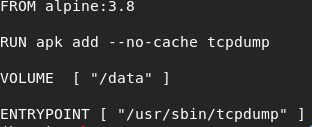
\includegraphics[width=0.5\textwidth]{dockerfile.png}
\caption{Basic Dockerfile for Tcpdump Container}
\end{figure}

  
  
\paragraph*{Docker Hub}
   The Docker software platform includes a cloud-based repository called the Docker Hub \cite{dockerhub} which allows users to download and build open source images on their local computers. At the time of writing, nearly 2.5 million images are available from Docker Hub. These include various operating systems --- such as Ubuntu,  Debian and Alpine --- and software packages --- such as Apache, Nginx and MongoDB. However, we avoid downloading images from Docker Hub as this introduces massive security risks; we can't verify the contents of these binaries and malicious actors have previously spread malware via Docker Hub \cite{dockermalware}. Instead, many images on the hub are built from linked, open-source repositories on Github. We limit ourselves to these images as we can build from the source Dockerfiles ourselves.

\paragraph*{Docker Networking} Upon installation, Docker automatically creates three networks: \textit{None}, \textit{Host} and \textit{Bridge}. Of these networks, only the Bridge network is of any relevance for this project as it allows us to securely run Docker containers with networking capabilities and in isolation. Containers attached to the Bridge network are assigned an IP address and are able to communicate with any other container on the network. We can create our own user-defined Bridge networks, which Docker's documentation recommends as it provides greater isolation and interoperability between containers \cite{docker_docs}. Furthermore, this allows us to set the subnet and gateway for our networks as well as the IP addresses of our containers, which simplifies scripting our scenarios considerably.


\paragraph*{Docker-Compose Files}

   Often, applications built using the Docker framework need more than one container to operate --- for example, an Apache server and a MySQL server running in separate containers --- and it is therefore necessary to build and deploy several interconnected containers simultaneously. Docker provides this functionality via \texttt{docker-compose}, a tool that allows users to define the services of multiple containers as well as the properties of their virtual network in a YAML file. By default, this file is named \textit{docker-compose.yml}. This allows for numerous containers to be started, stopped and rebuilt with a single command. We can also make some limited modifications to our images in the YAML file, such as sharing volumes, exposing ports and adding commands to be run on start up. Due to the ease of starting several containers at once as well as defining their behaviour from a single docker-compose file, this will be our primary method of deploying our containerised scenarios. We include an example docker-compose file below.
   
   \vspace{10mm}

  \begin{minted}[
    gobble=4,
    frame=single,
    linenos
  ]{yaml}
    version: '3'
    services:
      ping: 
        image: 'detlearsom/ping'
          container_name: ping-container
          environment:
            - HOSTNAME=google.com
            - TIMEOUT=2
      tcpdump:
        image: 'detlearsom/tcpdump'
          volumes:
            - '\$PWD/data:/data'
          command: not(ip6 or arp or (udp and (src port 5353 or 
                   src port 57621))) -v -w 
                   "/data/dump-010-ping-\${CAPTURETIME}.pcap"
          network_mode: 'service:ping'
  \end{minted}


\section{Malicious Behaviour and its Detection}


\textit{Malicious behaviour} can approximately be defined as any unwanted action or sequence of actions that threatens the availability, confidentiality or integrity of a user's data or hardware. Generally, computers and networks are secured against malicious behaviour by having systems in place that attempt to verify a user's identity before authenticating them at a given level of privilege. A user that bypasses this somehow is said to be an \textit{intruder} or \textit{attacker} of the computer system or network.

These protections are further fortified using a variety of technologies for preventing and detecting malicious behaviour. \textit{Firewalls} prevent malicious actors from accessing a network by blocking network connections according to predefined rules. In contrast, \textit{Intrusion Detection Systems} (IDSes) monitor network traffic to identify and stop intrusions that have successfully breached the network. 

Prior to the development of machine-learning-based software for the detection of malicious behaviour, intrusion classification techniques could be split into two broad categories: signature-based methods and anomaly-based methods. These methods attempt to classify intrusions based on a series of manually coded criteria. For signature-based methods, this involves classifying actions as malicious if they look sufficiently similar to previous described malicious actions \cite{vaidya2001dynamic}. In contrast, anomaly-based methods involve defining the bounds of acceptable behaviour for a computer system and flagging any behaviour that defies those boundaries \cite{garcia2009anomaly}. 

There are myriad ways in which a malicious actor can violate the security of a computer system or network and so there are numerous ways in which signature-based and anomaly-based detectors fail to accurately classify malware. Anomaly-based methods generalise better, more frequently preventing as-of-yet undefined malicious behaviour from occurring. However, they are more prone to false positives, potentially disrupting the execution of benign agents or software. Conversely, signature-based methods often fail to generalise, allowing novel exploits to bypass the detector and wreak havoc.

Furthermore, the intrusion ecosystem is constantly evolving, with various exploits and vulnerabilities continually coming into existence. Because of this, although IDSes perform highly when first tested, often with levels of accuracy exceeding 95\%, their performance often degrades with time as new exploits are developed or discovered \cite{chen2016more}. The definitions dictating the behaviour of anomaly-based and signature-based detectors must be repeatedly updated.

We need to develop \textit{robust} intrusion detection techniques that are capable of learning a more general notion of what it means for an actor to be in violation of the security of a system.  Machine learning techniques appear to be a natural candidate for such a classifier and, as such, most research in recent years has been focused on the development of machine-learning-based IDSes.

\subsection{Machine learning-based techniques}

A wide variety of machine learning-based intrusion detection systems have been published including Naive Bayes \cite{panda2007network} , Random Forests \cite{zhang2005network} and Neural Networks \cite{lee2001training}. Although these methods vary in their implementation, accuracy rates are broadly consistent across the algorithms with the previously cited papers reporting accuracies of 97.78\%, 94.8\% and 100\% respectively.   Instead, in order to optimise performance and robustness, it is necessary to choose informative and discriminating features.

The use of machine-learning techniques for the purposes of intrusion detection has been criticised. Although machine-learning classification has seen a great deal of success in other fields of research, such as computer vision and spam detection, Sommer et al. \cite{sommer2010outside} identify several manners in which machine learning-based intrusion detection differs from these other areas in a way that reduces its effectiveness. Primarily, Sommer et al. purport that although machine-learning techniques have seen a great deal of success in identifying \textit{similarities} between data, the concept of identifying \textit{abnormalities} in data, as an IDS is expected to do, is a similar but distinct task. Moreover, they claim that it is difficult to develop a machine learning-based IDS that can recognise the fundamental difference between an \textit{unusual} behaviour, which may be entirely benign, and \textit{malicious} behaviour, a subset of unusual behaviour that is actively trying to harm the system.

\subsection{Existing Datasets \& Criticism}
\label{sec:datasets}
There are already some datasets containing a mixture of benign and malicious traffic to test and train machine-learning approaches, captured using tools such as \texttt{tcpdump} or Wireshark. Such datasets attempt to emulate the network patterns found in 'real-world' internet traffic in order to provide researchers with a reasonable approximation of how a malware classifier may perform when deployed in a public environment. However, the development of such datasets are marred by several difficulties and have seen a wealth of criticism. As discussed by Sperotto et al. \cite{sperotto2009labeled}, simply monitoring the usage of several internet users and collecting the resultant traffic into a single dataset, although possible, introduces serious ethical concerns due to the large amount of sensitive or personally identifiable information that average internet users transmit during daily use --- such as passwords, GPS coordinates, private material.

To avoid this complication, researchers often use statistical approximations of real-world traffic to build such datasets. However, it is unclear to what extent such approximations actually resemble real-world traffic. For instance, it is unclear what the ratio of benign to malicious traffic should be as it is unknown what this ratio is in the real-world. Allix et al. \cite{allix2014machine} claim that the standard work-flow for developing machine-learning systems --- namely, collecting large amount of data and then training the algorithm on that data --- is necessarily flawed when applied to the domain of intrusion detection. They contend that the inherent secrecy of the intrusion ecosystem and the rate at which it develops make it is impossible to develop a dataset containing, say, network traces of intrusions that are currently being deployed by malicious agents. Instead, one can only build a dataset containing previously discovered attacks. As such, they suggest that it is impossible to release a static dataset that is truly representative of the real-world, impeding the performance of machine-learning-based classifiers.

Furthermore, many network traffic datasets are not comprehensively labelled. Even if only a single process is initiated by the user, VMs generate additional traffic from a variety of background processes, such as software querying servers to check for updates, resulting in aggregated application flows between processes. This necessitates the use of ground truth generation tools to classify flows. However, current methods of establishing the ground truth of network traffic datasets are well-known to be fallible\cite{carela2014our}. These are port-based methods, which classify traffic flows based on their port numbers, and deep-packet inspection (DPI) based methods, which classify flows based on analysis of their packet payloads. Port-based methods are unreliable due to the dynamic allocation of ports, several services sharing the same port and processes running on atypical ports. Moreover, although DPI-based methods are capable of inspecting the entirety of a packets contents, their performance has also shown to be lacking. Bujlow et al. \cite{bujlow2013comparison} have shown that many commonly used DPI-based methods for ground-truth generation fail to classify packets, with some methods failing to classify common protocols such as HTTP and FTP with less than 10\% accuracy. In contrast, it is trivial to produce a fully-labelled dataset from our Docker framework.

CIC-IDS 2017 \cite{sharafaldin2018toward}, released by the Canadian Institute for Cybersecurity, is the primary dataset that we shall compare our results to. The dataset was created by monitoring the network activity of several virtual machines running a series of scripted scenarios. The majority of these virtual machines produced exclusively benign traffic whilst others were designated as attackers, producing malicious traffic. Moreover, the exploit scenarios contained within the dataset are moderately recent, including botnets, cross-site scripting attacks and SQL injections. Furthermore, the dataset is far larger than many similar datasets, consisting of five sub-datasets captured over the course of a working week. Capturing traffic over such a lengthy period of time allows for the temporal development of attack scenarios to take place over several days, more accurately mimicking an intruder's movement through the network. CIC-IDS 2017, however, does not address the problems discussed in this section.


\subsection{Packet Inter-Arrival Times}
\label{sec:IATs}
We introduce the notion of packet inter-arrival times (IATs), defined as the time between sequential packets, as this will form a fundamental part of demonstrating that our Docker framework is capable of producing data that resembles real-world traffic.  The statistical distribution of packet inter-arrival times is dependant on the quality of the network and, as such, the distributions used to model network traffic have evolved as network bandwidth speeds have improved. Although early research focused on modelling network traffic via a Poisson distribution \cite{frost1994traffic} , such techniques have lost their relevancy as analysis of packet IATs has improved. In particular, experimental results suggests that the IATs of network packets follow a \textit{heavy-tailed} distribution that exhibits \textit{self-similarity} \cite{feldmann2000characteristics}. These terms are defined as follows: given a non-negative random variable $X$, it's distribution $F(x) = P(X \leq x)$ is said to be \textit{heavy-tailed} if $\hat{F} = P(X > x)> 0$ and $\forall x, y \geq 0$ then 

$$lim_{x \rightarrow \infty} P(X > x + y | X > x) = lim_{x \rightarrow \infty} \frac{\hat{F}(x + y)}{\hat{F}(x)} = 1 $$ 

Furthermore, given a zero-mean, stationary time series $X = (X_t; t = 1, 2, 3 ...)$, the m-aggregated series $X^{(m)} = X^{(m)}_k; k = 1, 2,  3 ...)$ is defined by summing $X$ into non-overlapping blocks of length $m$. We then say $X$ is H-self-similar if

$$X_t := m^{-H} \sum_{i = (t-1)m+1}^{tm} X_i \forall m \epsilon N $$
That is, $X$ is H-self-similar if each sub-distribution $X_{m}$ has the same distribution as $X$ when scaled by $m^H$.

In particular, Paxson et al. \cite{paxson1995wide} demonstrated that non-self-similar distributions fail to account for the 'burstiness' of network traffic as self-similarity is a necessary property to allow for network bursts of arbitrary length to occur.
The following self-similar, heavy-tailed distributions are typically used to model traffic in a modern setting:

\vspace{5mm}

\textbf{Pareto Distribution}: $$ \hat{F}(x) = x ^{-\alpha}, \alpha > 0$$

\textbf{Weibull Distribution}: 

$$ \frac{b}{a} (\frac{x}{a})^{b-1} e^{\frac{-x}{a}}^b $$
where a and b are defined as the scale and shape parameters respectively. In particular, there is considerable experimental evidence suggesting that the Weibull distribution is better than the Pareto distribution at modelling packet IATs \cite{arfeen2013role} \cite{arshadi2011tcp} . We use these distributions in section \ref{sec:exp1} to model artificially generated traffic.



%----- David said that I need a section on Related work on Infrastructure for Traffic Capture (Sandia Labs, Chemring Pattern of Life, hardware traffic generators?)




\chapter{Design \& Implementation of Docker Containers}
\label{sec:designandimp}

\section{Requirements}
\label{sec:require}

The primary task of this project is to develop a suite of Docker containers capable of producing traffic suitable for training a machine-learning-based intrusion detection system.  For each Docker container, we want a series of corresponding \textit{capture scenarios}. Running a given capture scenario triggers the creation of several Docker containers, each with a scripted task specific to that capture scenario. For example, a capture scenario may consist of a containerised client pinging a containerised server. Furthermore, we ensure that each Docker container in a scripted scenario that either produces or receives traffic will be partnered with a \texttt{tcpdump} container, allowing us to collect the resulting network traffic from each container's perspective automatically. We wish to publish this framework to a wider audience, allowing for further modification. To achieve this goal, we introduce the following key design principles:

\begin{itemize}

  \item Requirement 1 - To ensure that we produce representative data for modelling, we want the traffic generated by our container suite to consist of a good number of protocols that are commonly found in real-world traffic and existing datasets.
  
  \item Requirement 2 - For each protocol, we want to establish several capture scenarios  to encompass the breadth of that protocol's possible network traces. For instance, if we consider a capture scenario consisting of a client downloading various webpages over SSL, it is not enough to only include traffic from successful connections. We must also include several scenarios where the client fails to download the aforementioned webpage because of a misspelled address or missing certificate. Whenever possible, we also want to capture WAN traffic.
  
  \item Requirement 3 - For malicious traffic, we want to ensure that the attacks are varied, both in purpose and in network footprint, and relatively modern.
 
  \item Requirement 4 - We want the capture scenarios to be, on some level, deterministic. We discuss what it means for a scenario to be deterministic in section \ref{sec:deterministic}. 

  \item Requirement 5 - Once a capture scenario is initiated, we want to ensure that the scenario plays out with no further interaction from the user.
  
  
\end{itemize}

\section{Design for Requirements}

\subsection{Requirement 1 - Coverage of Protocol Types}
\label{sec:bro_logs}
As discussed previously, our primary aim is the development of a network traffic dataset for training IDSes. Therefore, in deciding how we should expand the Detlearsom benign scenarios, we initially investigated the protocols and applications present in existing network traffic datasets. Our analysis included CIC-IDS 2017 \cite{sharafaldin2018toward}, UNSW-NB15 \cite{moustafa2015unsw}, ICSX Botnet \cite{beigi2014towards} and Mawi \cite{fontugne2010mawilab}. We chose these datasets as they provide .pcap files of their network traffic which enables us to more easily see what protocols are present. To do this, we used the Bro IDS tool to generate log files, listing the results in table \ref{tab:results-bro}.


\begin{table}[ht!]
\begin{center}
\begin{small}
\begin{sc}
\begin{tabular}{ccccc}
\hline
\abovespace\belowspace
Protocol & UNSW-NB15 & ISCX & CIC-IDS 2017 & Mawi (2019-7-31)\\
\hline
\abovespace
HTTP         & 196195          & 2372        & 276405   &           156179   \\
SSL          & 540          & 141         & 285760     &      591551      \\
DNS          & 372748          & 200009          & 1820105      &    1581858      \\
X509          & 459          & 331          & 2758590      &     Unknown     \\
FTP          & 111685         &  1989         & 5540        &   278    \\
SSH          & 31320          & 434       & 5600         &   5503    \\
IRC          & 202          &  27       & 0          &    Unknown  \\
\belowspace
SMTP          & 44455         & 125         & 0      &      4601   \\
\hline
\end{tabular}
\end{sc}
\end{small}
\vskip -2mm
\caption{Bro Log Flow Count}
\label{tab:results-bro}
\end{center}
\vskip -4mm
\end{table}

The protocols listed in table \ref{tab:results-bro} make up over 90\% of the benign traffic in these datasets. Moreover, although the ratio of protocols in datasets can differ significantly, we see some patterns: namely, protocols associated with general browser usage --- such as HTTP, SSL, DNS --- are the most common in each dataset. 

We could base the ratios of protocols in our own dataset off of those found in an existing dataset where the traffic has been artificially generated. However, this would be problematic. In the case of CIC-IDS 2017, some protocols that make up a substantial amount of real-world traffic are glaringly omitted --- such as bittorrent or video streaming protocols. In contrast, although UNSW-NB15 contains a better range of protocols, only a small percentage of their web traffic is transmitted over SSL which is completely unrepresentative of real-world traffic. Furthermore, in both these datasets, it appears that a non-negligible amount of traffic is the result of remote desktop protocols being used to interact with the virtual machines generating data, such as X11, VNC and RDP, which we consider to be unwanted noise. Instead, we opt to use these datasets as a rough guideline for constructing datasets but not closely following any one in particular.


\subsection{Requirement 2 - Variation within Protocols}

Often, datasets contain traffic from a given protocol but the manner in which that protocol in used is highly-restricted and it is unclear if this traffic is representative of its real-world equivalent usage. For instance, in CIC-IDS 2017 the vast majority of successful FTP transfers consist of a client downloading a .txt file containing the Wikipedia page for 'Encryption' several hundred times in a day. Therefore, it is possible that an IDS trained on CIC-IDS 2017 may trigger a false positive when, say, a larger file is downloaded over FTP due to the difference in the duration or backwards packet length of the flows. Moreover, we would hope that an IDS would be capable of detecting both successful and unsuccessful intrusions. We aim to avoid this problem, when applicable, by including several variations for a given protocol or scenario, including unsuccessful attacks.  

\subsection{Requirement 3 - Inclusion of Malicious Traffic}

To construct datasets which comprehensively describe anomalous traffic, our capture scenarios should contain a diverse range of attacks. To do this, we chose to incorporate exemplar attacks from a variety of attack types. Namely, we hope to include at least Denial of Service (DoS), Bruteforcing, Data Exfiltration, Botnets and Web attacks. We chose these categories as these attack types are commonly found in other datasets and have the potential to cause serious disruption to a system. Moreover, the network footprint of these attacks have a wide range; whilst a DoS attack may involve sending several gigabytes of traffic to a victim, a data exfiltration attack may involve sending only a single command.

\subsection{Requirement 4 - Deterministic Scenarios}
\label{sec:deterministic}

It is impossible to guarantee that each scenario will produce a truly 'deterministic', or repeatable, output due to  differences in network conditions, computational times and randomization. For instance, randomizing the order in which file transfers take place. However, it is important that each run of a scenario produces comparable results. We could describe the data produced by our scenarios as being 'reproducible' --- i.e. we allow for some margin of error between the datasets --- but this doesn't fully capture the property we desire. Instead, we aim for our data to be \textit{deterministic up to networking and computational differences}. This means that when running a scenario multiple times, we'd expect most equivalent packets to be largely identical, barring IATs i.e. they are deterministic up to \textit{networking} differences. However, we'd also expect periods of greater variation in packet IATs, sizes and content due to non-determinism in the underlying protocols such as, say, two runs of an SSH scenario exchange keys of different lengths i.e. they are deterministic up to \textit{computational} differences.

\subsection{Requirement 5 - Automated Capture}

It is relatively straightforward to automate the interactions between containers using the docker-compose file. The \texttt{volumes} command allows us to share scripts with each container and the \texttt{command} command allows us to execute them on container start-up. Although we can specify the order containers are started in using \texttt{depends\_on}, this sometimes is not enough to fully script a scenario. In these cases, we use \texttt{docker exec} to execute code during the operation of the container.



\section{Dataset Collection}
\label{dataset_require}
As discussed in section \ref{sec:datasets}, the datasets that are currently used to train and evaluate network intrusion detection systems are lacking. The dearth of quality datasets has been criticised by several commentators such as Tavallaee et al. \cite{tavallaee2009detailed} and Sommer et al. \cite{sommer2010outside}, the latter of which stated that the "most significant challenge an evaluation faces is the lack of appropriate public datasets for assessing anomaly detection systems". Due to the fact that static datasets reflect real-world anomalous traffic only for a brief time frame, Shiravi et al. \cite{shiravi2012toward} suggests that datasets should be dynamically generated allowing for new data to be introduced to maintain their longevity. We believe that a Docker framework adhering to the design principles outlined in section \ref{sec:require} reasonably fits these demands as it is possible to continually expand it by developing new scenarios. In a similar vain, Sommer et al. stress the importance of using multiple datasets with different attack patterns to evaluate the robustness of an intrusion detection system and its ability to detect as-of-yet unknown anomalies. Again, we feel as though the Docker framework addresses these concerns, as one can generate multiple datasets whilst have full control over the attacks and protocols contained within each.



Shiravi et al. identify five characteristics that are necessary for a dataset to be considered adequate. Namely, these are a realistic network and traffic, fully labelled intrusions, total interaction capture --- meaning that all traffic within LANs is captured ---, complete capture --- meaning that the dataset is free form any sanitation --- and diverse intrusion scenarios. These are the standards that we shall use to evaluate our dataset.

%----- Move some of this criticism to background section

\section{Implementation}

\subsection{Implementation of Tooling}

Because the network traffic between Docker containers takes place on an isolated, virtual network, the network conditions far exceed those found in the real-world. For instance, we measured network throughput across a docker bridge network using \texttt{iperf}\cite{iperf} and found that the bandwidth rate surpassed 90Gbits/s. 


\begin{figure}[h]
\centering
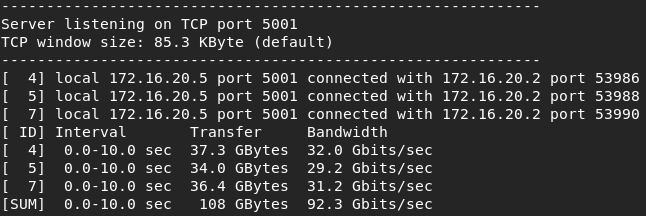
\includegraphics[width=0.5\textwidth]{screenshot.png}
\caption{Iperf output on a Docker bridge network with 3 parallel threads}
\end{figure}
\vspace{-5mm}
As such, it was necessary to develop scripts capable of emulating more realistic network conditions. This was possible using \texttt{tc-netem} \cite{tc-netem}, a suite of tools that expand the Linux traffic control facilities which allow for the addition of network delays, packet loss and rate limiting to a network interface. Although we could use tc-netem directly in order to apply these settings to the entire docker network, we felt that this didn't provide us with sufficiently granular control over each individual container as it would only allow us to apply the same settings to every single running container. Therefore, it was necessary to develop a series of wrapper scripts for each tc-netem command that would allow us to apply these settings to an individual container's virtual ethernet.

%Furthermore, although these tc-netem scripts allow us to alter the network conditions, these alterations are added entirely artificially. As such, we felt it would be prudent to develop some scripts capable of simulating poor network conditions in a more realistic manner. Therefore, we developed a simple mechanism using netcat to add 'real' network congestion to a Docker virtual network. Unfortunately, due to the incredibly high throughput of the Docker virtual networks, netcat is not optimised to consume sufficient bandwidth to markedly influence the Docker network. Instead, this tool must be used in conjunction with the above tc-netem scripts to rate limit the bandwidth to a more realistic speed before the effects of netcat congestion are noticeable.

  
\subsection{Prior Scenarios}



\begin{tabular}{ |p{2cm}||p{10cm}| }
 \hline
 Name & Description \\
 \hline
 Ping   & A client pinging a DNS server    \\
 Nginx &   A client accessing an Nginx server over HTTP and HTTPS   \\
 Apache & A client accessing an Apache server over HTTP and HTTPS \\
 SSH    & A client communicating with an SSHD server over SSH\\
 vsftpd &  A client communicating with a vsftpd server over FTP \\
 Scrapy & A client scraping the University of Edinburgh website  \\
 Syncthing& 3 clients synchronise files with one another via Syncthing\\
 mailx& A mailx instance that sends emails over SMTP \\
 IRC & 2 IRC clients communicate via an IRCd server \\
 \hline
\end{tabular}
 \captionof{table}{\label{tab:prev}}
 
Prior to my work on this project, several Docker containers with a very similar purpose to that of this dissertation were built as part of the Detlearsom project \cite{detlearsom}. These containers were designed to primarily produce network traffic data of fundamental internet protocols. Moreover, the network traffic generated by these container suites consisted of entirely benign traffic. The design of these containers broadly fit in with our design philosophy moving forward with the Detlearsom project and thus formed the bedrock of our work expanding the protocols and scenarios covered. These previous containerised scenarios are listed in table \ref{tab:prev}.



\subsection{Implementation Process}

The implementation process for our Docker containers followed broadly the same outline for each scenario. 

\begin{enumerate}

  \item Firstly, we draw up a broad outline of a given protocol, scenario or attack. We then identify the \textit{primary} container for a given scenario, which we defined as any containerised server and/or intentionally vulnerable application, before creating and building a Dockerfile containing all necessary dependencies. 
  
  \item We now run this container which allows us to develop the scripts necessary to enact the desired behaviour from the host machine. For instance, if the primary container is a vulnerable server and we want to capture the traffic from a DoS attack, we ensure that such an attack is possible by launching it from the host machine initially. 
  
  \item Having scripted the behaviour of the secondary containers from the host machine, we simply need to build Dockerfiles which download and install all necessary dependencies before transferring any scripts to their respective containers.

  \item We then create a docker-compose file that launches all containers simultaneously and executes all necessary commands. Finally, we develop a script that, upon running, calls this docker-compose file and allows the user to specify the various parameters of the scenario --- for instance, how many times a scenario should be run and how long each scenario should be run for.

\end{enumerate}

Following the Docker \textit{best practise} guidelines \cite{bestpractise}, each Docker container in our framework consists of a single service with a specialised purpose, with as few additional dependencies as possible. When possible, we will opt to use Alpine Linux as our base image to house our containers, which is far more lightweight than Ubuntu or Debian as this improves the scalability of our scenarios. Moreover, we ensure that there are minimal inter-dependencies between the containers of a scenario. This allows us to easily modify and update our containers as new versions of the underlying software are released with minimal interference with other containers.

  
    \subsection{Simple Example Scenario - FTP server}
              \begin{figure}[h!]
\centering
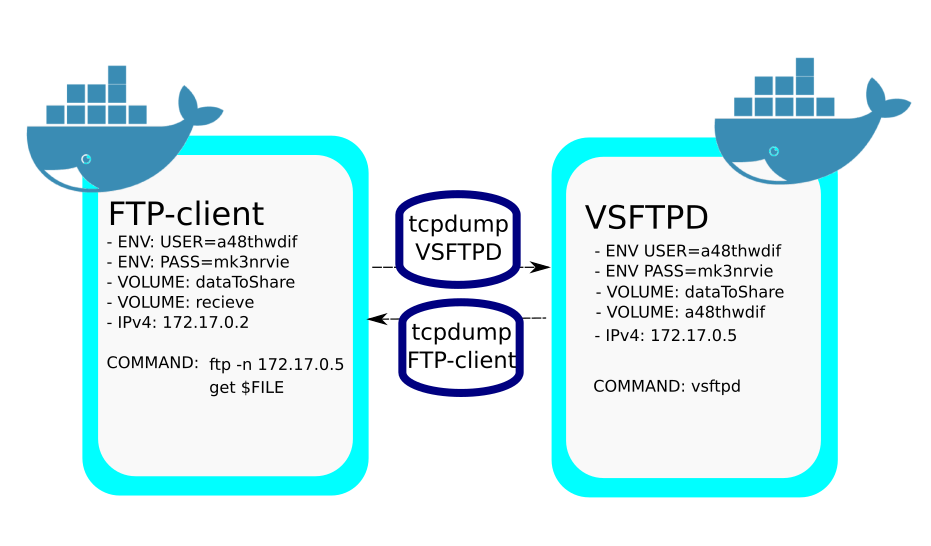
\includegraphics[width=0.50\textwidth]{ftp_example.png}
\caption{Diagram of our FTP scenario}
\end{figure}
    We shall review the design of a prototypical capture scenario, namely, an FTP server and client interaction. The entire interaction is initiated by a single script, which allows the user to specify the length of the interaction, the number of times the interaction takes place as well as the specific scenario that should govern the interaction at runtime. Upon specifying these parameters, the script then generates a random ftp username and password, creating the necessary \textit{User} directory on the host machine before calling the docker-compose file which creates a user-defined bridge network. Subsequently, the necessary containers are then started which, in this case, consist of a vsftpd server, a client with ftp installed and two containers running tcpdump to capture all of the traffic emitted and received by the client and server respectively into separate .pcap files. These .pcap files are then sent to the host machine via a shared data directory. In addition, the host machine also shares:
    
    \begin{itemize}
        \item A \textit{dataToShare} volume containing files that can be downloaded by the client.
        \item The \textit{User} directory with the server --- which contains the same files as the \textit{dataToShare} folder.
        \item An empty \textit{recieve} folder with the client into which the files will be downloaded.
        \item The random username and password is also shared with the client container to allow it to authenticate itself with the server.
    \end{itemize}
    
    Up to this point, no network traffic has been generated and the containers are now ready to begin communicating with one another. 
    For this particular interaction between an FTP server and client, we want to ensure that it is possible to capture the many ways in which an FTP session may develop. For instance, the client may seek to download files via the \texttt{get} command or the \texttt{put} command, alongside many other possibilities. There are 13 possible capture scenarios intended to encapsulate a wide range of potential FTP sessions. These include downloading a single file using \texttt{get} or \texttt{put}, downloading every file using \texttt{mget} or \texttt{mput}, deleting every file from the server and requesting files from the server without the necessary authentication.

    Finally, after the scenario ends, both the \textit{User} directory and any downloaded files are then removed from the host machine. Following this, the containers are then stopped and the bridge network is torn down. All necessary containers, volumes and scripts are in the same position prior to initiating the scenario --- barring any generated .pcap files --- allowing for the scenarios to be started repeatedly with minimal human interaction.
    
    \begin{figure}[H]
\centering
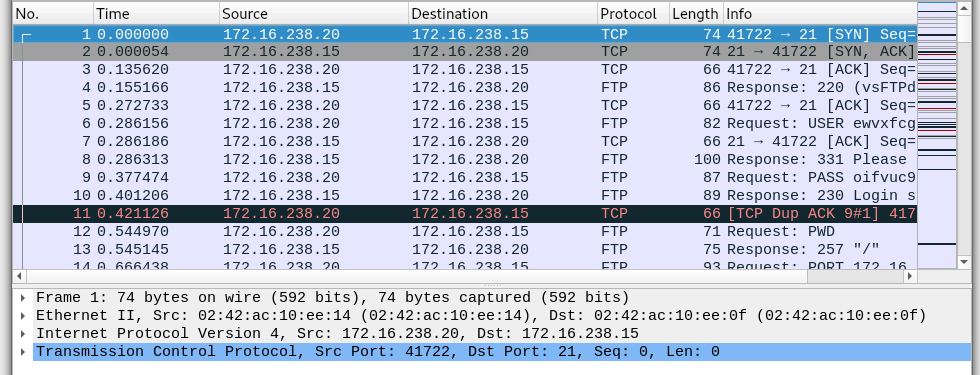
\includegraphics[width=0.75\textwidth]{pcap.png}
\caption{Wireshark view of a .pcap file from our FTP scenario}
\end{figure}
    

\subsection{Complex Example Scenarios - Secure SQL \& Insecure SQL}

We outline the implementation of two complex scenarios: a benign SQL scenario and a malicious SQL scenario. The benign scenario simulates the behaviour one would expect from a secure user registration page whilst the malicious scenario simulates a SQL injection attack. We include some necessary files and code snippets for the secure SQL scenario in Appendix A.
\paragraph*{Implementation of Secure SQL}
We discuss the implementation of our secure SQL scenario before describing how we modified this scenario to allow for SQL injection attacks. Upon starting our script, three primary containers --- a MySQL server, an Apache server and an 'Admin' user --- are launched alongside their respective tcpdump containers. For ease of communication, all the containers sit on the same subnetwork and are given fixed IP addresses.

Our MySQL server is built from the official docker-library/mysql Github repository. Upon starting our docker-compose file, we expose port 3306 --- the default for MySQL connections ---, we replace the preexisting configuration file with our own and we send the necessary scripts to build our MySQL database. Every time we start this container we are effectively starting MySQL for the very first time. As such, we wait 60 seconds until MySQL generates a random password for root access, which we extract from the container by monitoring its Docker log file. We can then create a database and table to store our user credentials in. The table has four columns: user id, username, password and timestamp. We demand that all usernames are unique and that neither the username nor password can be empty. 

We obtain our Apache Dockerfile from the officially maintained docker-library/PHP Github repository, modifying the Dockerfile slightly to enable the \texttt{mysqli} package. On launching this container, we expose port 80 to allow for HTTP connections and share a volume containing all our webpages. These include a configuration page which immediately starts a connection to the MySQL server, a registration Page, a login Page and an index page that a user is redirected to upon successfully logging in. All user data is handled using prepared statements according the standards set by OWASP \cite{owasp}, preventing SQL injection attacks.

Finally, our Admin user is an Alpine Linux instance with Python installed. We also install the \texttt{requests} library to communicate over HTTP. This container waits until the MySQL server is completely set up before registering users and sending their details to the login page. The usernames and passwords are drawn from a text file containing roughly 40000 strings. Although this is only a single scenario, we capture traffic from successful and unsuccessful logins and registrations, as well as all traffic between the Apache and MySQL containers.


\paragraph*{Implementation of Insecure SQL}

We modify the above containers to generate malicious traffic. For the MySQL server, instead of creating an empty database and gradually adding entries, we import a previously created user table that had been saved using the \texttt{mysqldump} command line tool. This is a critical design choice; we could have used the same technique as our secure SQL scenario to fill the user table but this is problematic. In particular, we would generate .pcap files with a mix of benign traffic from the normal registrations and malicious traffic from the injection attack.

For our Apache server, we modify the PHP code for the login page by removing all prepared statements, making these fields vulnerable to SQL injection. We keep the registration page identical, as this allows us to generate a traffic from failed attacks.

Finally, we replace our Admin user with an Attacker. This container operates in a similar manner, however, instead of entering valid usernames to the login fields, the Attacker enters a series of strings that result in unwanted behaviour. For instance, entering \texttt{ ' or 1=1-- } returns the entire database.


\begin{comment}
Given the above considerations, we ultimately ended up developing the following scenarios:

\begin{itemize}
    \item A bittorrent scenario - Consists of a host, a tracker and three clients. Torrents are shared from the host to the clients, who either download files from the host and then seed them or download from peers around the world.
    \item A secure SQL scenario - Consists of an admin, Apache server and SQL server. Users are added to an SQL database by the admin via the apache server. It's possible for the admin to register users as well as login and logout.
    \item An NTP scenario - Consists of an NTP server who synchronises its time with other NTP servers and a client who then, in turn, synchronises its time with this NTP server.
    \item A music streaming scenario - Consists of a Mopidy server and MPC client. The client connects to the server and then streams music in a variety of ways i.e randomly stopping and starting, playing through playlists in order, shuffling playlists etc.
    \item A video streaming scenario - Consists of an Nginx server, a 'streamer' user and a 'viewer' user. The streamer pushes a random video to the Nginx server, where the viewer then connects and watches it over RTMP.
    \item A wget over WAN scenario - Consists of a series of wget clients. The clients use wget to randomly scrape one of the 10000 most popular websites, posing as a variety of user-agents and allows for downloads over HTTP or HTTPS.
    \item An SSH bruteforcing scenario - Consists of a sshd server and a malicious client running patator. The client repeatedly attempts to guess the password of a user. The attack can succeed or fail.
    \item A URL fuzzing scenario - Consists of an Apache server and a malicious client running patator. The client repeatedly guesses and attempts to connect to possible webpages, which may contain sensitive information.
    \item A Goldeneye DoS scenario - Consists of an Nginx server and a malicious client running Goldeneye. The client initiates a DoS attack against the server. 
    \item A Slowhttptest scenario - Consists of an Apache server and a malicious client running Slowhttptest. The client can initiate a variety of DoS attacks against the server.
    \item An insecure SQL scenario - Same as the secure SQL scenario above, but also consists of a malicious client. The client waits a certain amount of time before attempting to exfiltrate the entire SQL database via an SQL injection fuzzing attack. The attack can succeed or fail.
    \item A basic authentication bruteforce scenario - Consists of an Apache server that denies access to anyone without the proper credentials and a malicious client. The client attempts to brute force access to the server. The attack can succeed or fail.
    \item A DDoS scenario - Consists of an Apache server, a Mirai CNC server, 3 Mirai bots and an attacker. The attacker connect to the CNC server via Telnet and then initiates a DDoS attack against the Apache server. A variety of DDoS attacks are possible.
    \item A heartbleed scenario - Consists of an Apache server and a malicious client. The Apache server is running a version of OpenSSL that is vulnerable to the Heartbleed attack which the client exploits via Metasploit.
    \item A backdoored server scenario - Consists of an Nginx server that has an Ares backdoor installed, an Ares CNC server and an attacker. The attacker connects to the CNC server, where they can then launch an attack.
    \item A Cryptojacking scenario - Same as the above backdoored scenario, but allows the attacker to surreptitiously install a Cryptocurrency mining service.
    \item An XXE scenario - Consists of an Apache server and a malicious client. The Apache server is configured to allow XXE attacks, enabling the malicious user to read sensitive files or inject certain commands.
\end{itemize}

\end{comment}


\section{Creation of Datasets}
\label{sec:dataset_create}

In contrast to how many other network traffic datasets were created, it's unfeasible to have all of our Docker scenarios running simultaneously over a large period of time. This is both due to personal hardware constraints as well as networking limitations of the Docker framework --- such as clashing IP addresses and ports. The data for our datasets was collected over the course of several weeks before being coalesced into a main dataset. If done naively, this presents a problem. As discussed by Shiravi et al. \cite{shiravi2012toward}, it is unclear whether randomly merging both attack and benign data in an overlapping manner introduces inconsistencies to the data. Therefore, we created our dataset by collecting data in 10000 second chunks, where both benign and attack scenarios are activated via human interaction. All .pcap files collected during a given chunk can then be merged together in a manner that ensures that the collected traffic is as consistent as possible --- which may not happen if attacks were inserted randomly. We then stitch together all of these chunks into a single .pcap file using a combination of \texttt{Mergecap} \cite{mergecap} and \texttt{Editcap} \cite{editcap}. This allows us to shift the timings of each .pcap file by a fixed amount such that all of are chunks occur in succession whilst maintaining the internal consistency of each chunk.

With respect to the problem of labelling, ensuring that each Docker container only produces network traffic related to a single protocol or process is a fundamental design choice as it allows us to build a dataset with a perfectly accurate ground truth of application flows --- that is to say, we can guarantee the process or protocol producing any packet in our dataset. 

In designing our dataset, we largely followed the lead of existing datasets. Namely, the Bro logs produced in section \ref{sec:bro_logs} gave us a reasonable approximation of the number of flows of a given protocol and their respective ratios. As previously discussed, HTTP, SSL, DNS and x509 made up the bulk of these datasets and, as can be seen from table \ref{tab:results-bro}, there was then consistently a large gap between these and other common protocols. Unfortunately, some of our data generating scenarios do not produce a fixed number of flows. As such, maintaining a desired ratio between protocols when constructing our dataset, although possible, was largely the result of trial and error.



\begin{landscape}
\begin{comment}
\centering
\section{Implemented Scenarios}


\begin{tabular}{ |p{3cm}||p{12cm}|  p{2.75cm} | p{.4cm} |  p{.4cm} | }
 %\hline
 %\multicolumn{5}{|c|}{} \\
 \hline
 Name & Description  & Attack Type & \#S & \#C \\
 \hline
 Bittorrent   & A host downloading and seeding torrents to local and remote clients. & Benign   & 3  & 10 \\
 Secure SQL &  An admin adds users to a MySQL database via an Apache Server. & Benign & 1 & 6 \\
 NTP & An NTP client resets container clock via remote NTP servers. & Benign & 1 & 4 \\
 Music Stream    & An MPC client streams music from a Mopidy server. & Benign  & 5 & 4 \\
 Video Stream &  A streamer uploads video to an Nginx server where a viewer watches it.& Benign  & 1 & 6\\
 Wget over WAN & A client recursively download random websites. & Benign &  5 & 2 \\
 SSH Bruteforce & A malicious user bruteforces a password over SSH.  & Bruteforce & 3 & 4\\
 URL fuzzing & A malicious user fuzzes a webpage looking for hidden webpages. &  Bruteforce & 1 & 4 \\
 Basic Bruteforce & A malicious user bruteforces a password over Basic Authentication. & Bruteforce & 2 & 4 \\
 Goldeneye DoS & A malicious users tries to knock a webserver offline with Goldeneye. &  DoS & 1 & 4\\
 Slowhttptest DoS &  A malicious users tries to knock a webserver offline with Slowhttptest.  & DoS & 4 & 4\\
 Mirai & A Mirai botnet launches a DDoS attack against an Apache server. &Botnet/DDoS & 1 & 12\\
 Heartbleed & A malicious user exfiltrates data via the Heartbleed exploit.  & Exfiltration & 1 & 4\\
 Ares & A malicious user exfiltrates data via a backdoor on an Nginx server. &  Exfiltration & 3 & 6\\
 Cryptojacking & A malicious user installs cryptomining software on a backdoored server. & Cryptojacking & 1 & 6\\
 XXE & A malicious user exploits a faulty XML parser & Web Attack & 3 & 4\\
 Insecure SQL & A malicious user exploits a SQL injection leading to data leakage.  & Web Attack & 2 & 6\\
 \hline
\end{tabular}
\hspace{30mm} Note: S\# is the number of individual scenarios of a simulation. C\# is the total number of containers used in a simulation.
\end{comment}

\centering
\section{Implemented Scenarios}


\begin{tabular}{ |p{3cm}||p{6cm}| {p6cm} | p{2.75cm} | p{.4cm} |  p{.4cm} | }
 %\hline
 %\multicolumn{5}{|c|}{} \\
 \hline
 Name & Description & Tools/Software Used & Attack Type  & \#S & \#C \\
 \hline
 Bittorrent   & Download and seed torrents. & Transmission, Opentracker & Benign   & 3  & 10 \\
 Secure SQL &  Apache with MySQL. & PHP, MySQL, Apache & Benign & 1 & 6 \\
 NTP & An NTP client. & NTPD & Benign & 1 & 4 \\
 Mopidy    & Music Streaming. & MPC, Mopidy & Benign  & 5 & 4 \\
 RTMP & Video Streaming Server.& RTMPdump, Nginx RTMP, ffmpeg & Benign  & 1 & 6\\
 Wget over WAN & Download random websites. & Wget & Benign &  5 & 2 \\
 SSH Bruteforce & Bruteforcing a password over SSH. & Patator, SSHD & Bruteforce & 3 & 4\\
 URL fuzzing & Bruteforcing URL & Nginx, Patator & Bruteforce &  1 & 4 \\
 Basic Bruteforce & Bruteforcing Basic Authentication. & Nginx & Bruteforce & 2 & 4 \\
 Goldeneye DoS & DoS attack on Web Server & Goldeneye, Apache &  DoS & 1 & 4\\
 Slowhttptest DoS &  DoS attack on Web Server & Slowhttptest, Nginx & DoS & 4 & 4\\
 Mirai & A Mirai botnet DDoS. & Mirai bots, Mirai CnC, Telnet &Botnet/DDoS & 3 & 12\\
 Heartbleed & Heartbleed exploit. & msfconsole, Apache, OpenSSL  & Exfiltration & 1 & 4\\
 Ares & Backdoored Server. & Ares CnC, Apache &  Exfiltration & 3 & 6\\
 Cryptojacking & Cryptomining malware. & Ares CnC, Apache, CNRig & Cryptojacking & 1 & 6\\
 XXE & External XML Entity & PHP, Apache & Web Attack & 3 & 4\\
 Insecure SQL & SQL injection attack & PHP, MySQL, Apache & Web Attack & 2 & 6\\
 \hline
\end{tabular}
\hspace{30mm} Note: S\# is the number of individual scenarios of a simulation. C\# is the total number of containers used in a simulation.



\end{landscape}



\chapter{Experimentation}
\label{sec:experiments}
\section{Experimental Design}

To evaluate the utility of our Docker framework, we construct a series of experiments. We had two specific goals in mind when designing our experiments. Firstly, we wanted to demonstrate that the traffic generated by our Docker scenarios is meaningfully useful for training and testing intrusion detection systems so it must be sufficiently representative of real-world traffic. Secondly, we wanted to demonstrate that having a framework to continually generate data is extremely useful for evaluating the efficacy of intrusion detection systems.


\begin{comment}

In order to properly classify internet traffic --- either into discreet application flows or for the purposes of intrusion detection ---, it is necessary to consider a comprehensive range of features. Of these features, the inter-arrival times (IATs) of packets has been shown to be of considerable importance. In particular, Jaber et al. \cite{jaber2011can} demonstrated that a k-means classifier is capable of segregating traffic flows into application flows based solely on packet inter-arrival times with high efficacy, achieving an accuracy exceeding 90\%. Moreover, packet inter-arrival times are a useful feature for anomaly detection systems, particular in the realm of APT and DoS detection. For instance, Berk et al. illustrated how attackers can artificially delay packets in order to exfiltrate data from a network and, as such, covert channels of communication can be detected via the unusual distribution of packet inter-arrival times. Furthermore, Arshadi et al. \cite{arshadi2011tcp} found that certain classes of malware, namely worms and trojans that initiate their attacks through unusual port connections can be detected through analysis of packet inter-arrival times. As such, in order to generate a dataset for the purposes of intrusion detection, it is necessary to ensure that our packet arrival times are distributed in a manner that is representative of real-world packet times. However, it is not immediately clear if the traffic generated by our suite of Docker containers satisfies this condition. Namely, a considerable percentage of the traffic generated by our docker containers is transported over the Docker virtual network and so an insignificant percentage of our packets succumb to problems associated with normal network congestion, such as packet loss, corruption and packets arriving out of order. However, over the course of developing the Docker scenarios, we developed wrapping scripts that allow us to artificially add such phenomena via tc-netem to our generated traffic, but, again, it is unclear whether such network emulation actually provides us with data that could plausibly come from real-world traffic. Therefore, we devote considerable time to demonstrating that it is possible for traffic generated by our Docker suite to conform to real-world distributions when altered using tc-netem. 

\end{comment}

\begin{comment} 
 
\begin{figure}[h!]
\caption{Weibull Probability plot of IATs of MAWI dataset}
\centering
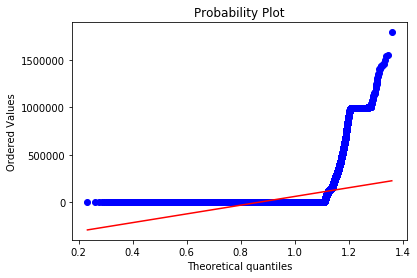
\includegraphics{mawi_probplot.png}
\end{figure}

\begin{figure}[h!]
\caption{Weibull Probability plot of IATs of CIC-IDS dataset}
\centering
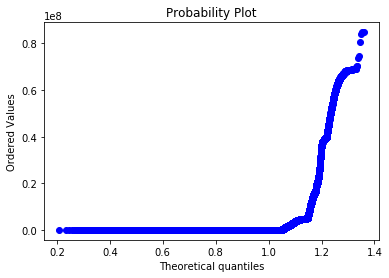
\includegraphics{weibull_prob_plot_cic_ids.png}
\end{figure}


\begin{figure}[h!]
\caption{Weibull Probability plot of IATs of UNSW dataset}
\centering
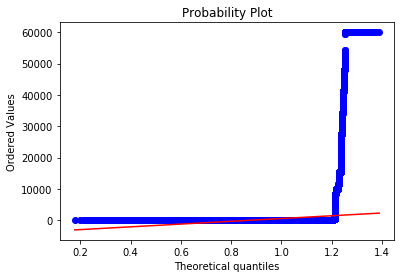
\includegraphics{unsw_probplot_all_data.png}
\end{figure}

\begin{figure}[h!]
\caption{Weibull Probability plot of IATs of benign data in UNSW dataset}
\centering
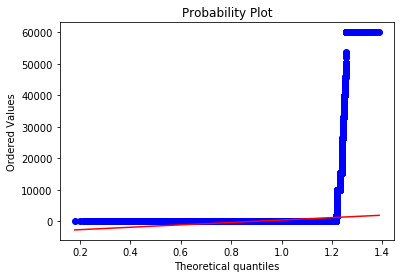
\includegraphics{unsw_probplot_ben_data.png}
\end{figure}

\begin{figure}[h!]
\caption{Weibull Probability plot of IATs of malicious data in UNSW dataset}
\centering
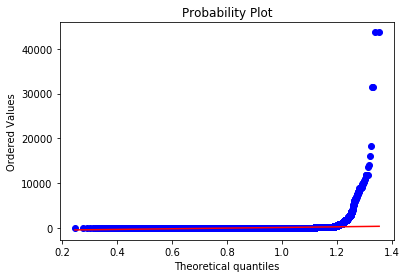
\includegraphics{unsw_plobplot_mal_data.png}
\end{figure}

\begin{figure}[h!]
\caption{Exponential Probability Plot of IATS in UNSW dataset}
\centering
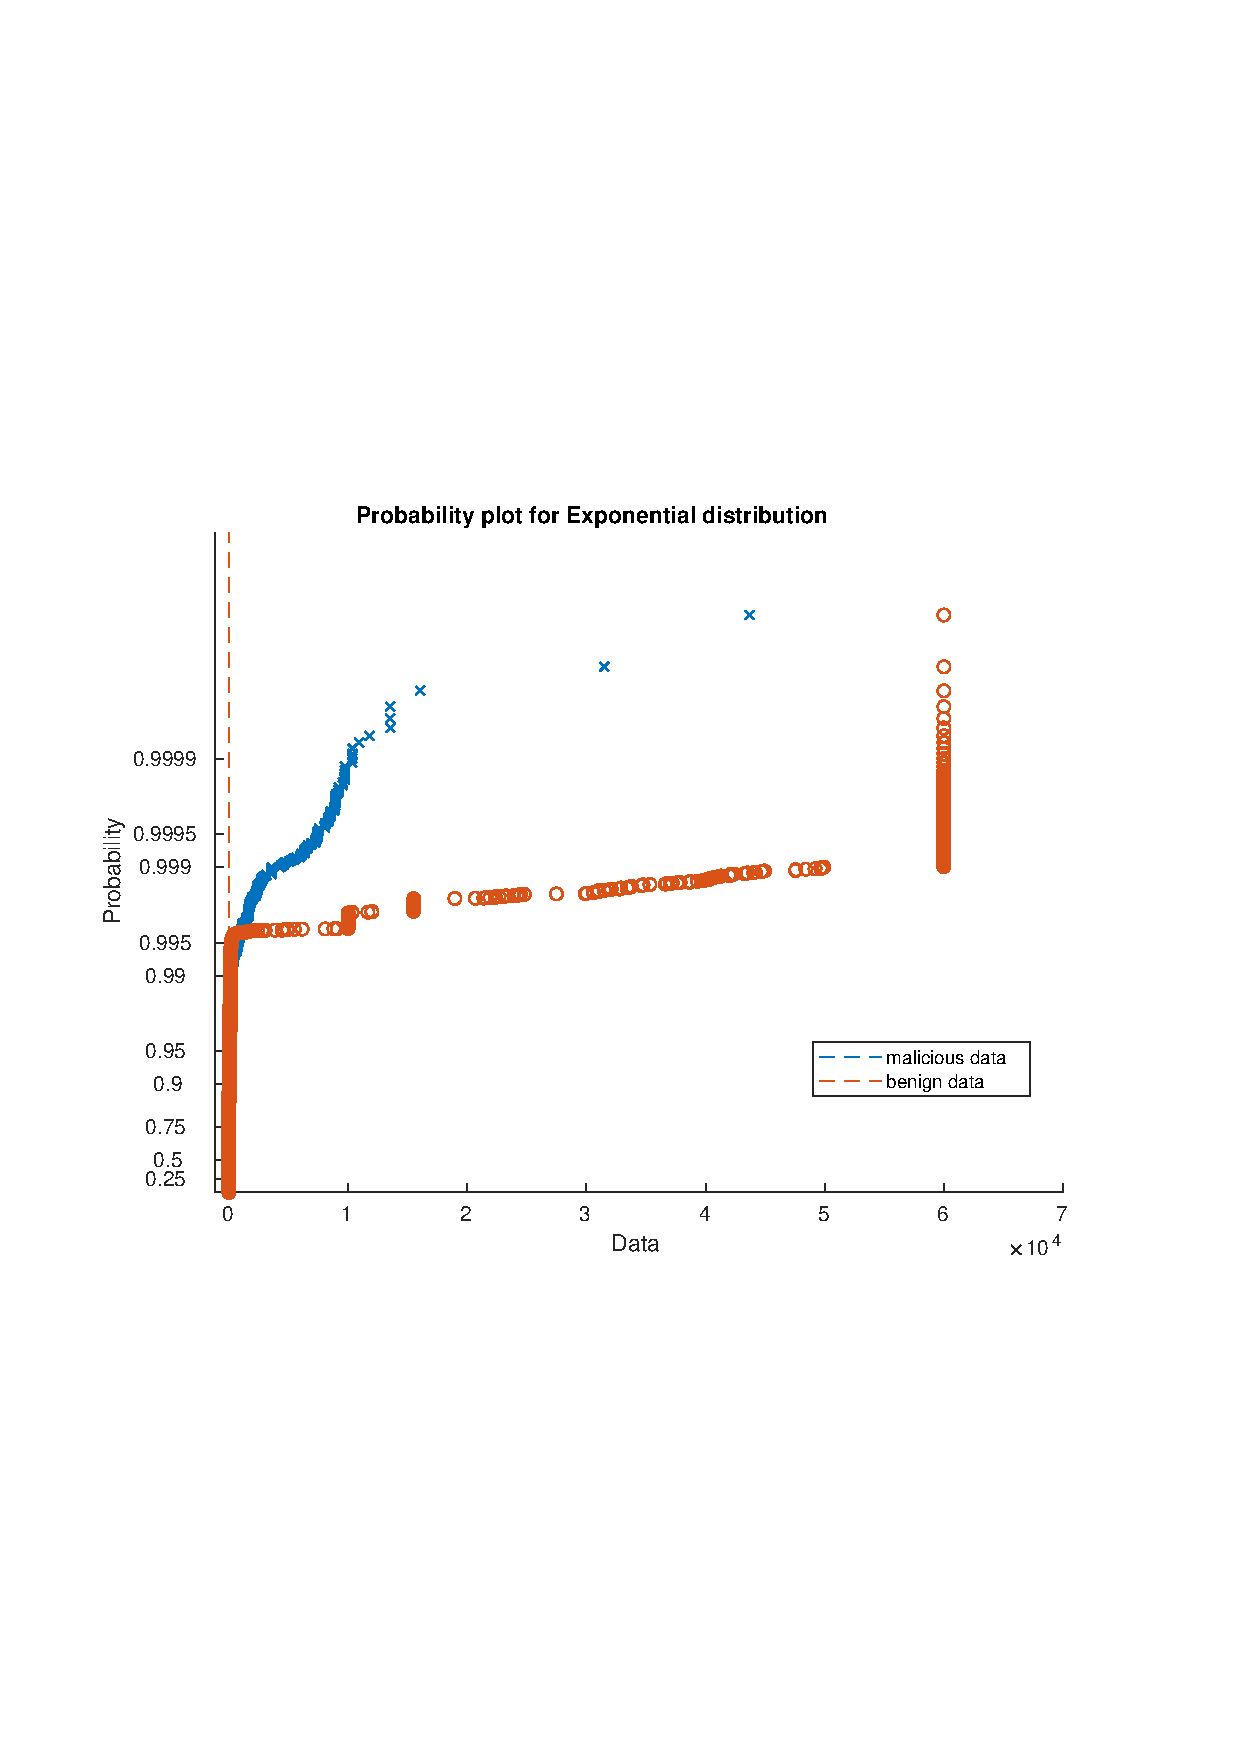
\includegraphics[scale=0.6]{UNSW_ben_vs_mal.pdf}
\end{figure}

\end{comment}



\section{Experiment 1: Exploration of Artificial Delays}
\label{sec:exp1}

\subsection{Motivation}

We devote considerable time to demonstrating that it is possible for traffic generated by our Docker suite to conform to real-world distributions when altered using \texttt{tc-netem}. To properly classify internet traffic --- either into discreet application flows or for the purposes of intrusion detection --- it is necessary to consider a comprehensive range of features. Of these features, the inter-arrival times (IATs) of packets has been shown to be particularly relevant \cite{zander2005automated} \cite{nguyen2008survey}. Moreover, packet inter-arrival times are a useful feature for anomaly detection systems, particularly in the realm of data exfiltration and DoS detection \cite{iorliam2016flow}. For instance, Berk et al. \cite{berk2005detection} illustrated how attackers can artificially delay packets to exfiltrate data from a network; such covert channels of communication can be detected via the unusual distribution of packet inter-arrival times. Arshadi et al. \cite{arshadi2011tcp} found that certain classes of malware, namely worms and trojans that initiate their attacks through unusual port connections can be detected through analysis of packet inter-arrival times. Therefore, in order for IDSes trained on our Docker traffic to be effective, it is vital that the IATs of these packets are realistic.

However, it is not immediately clear if the traffic generated by our suite of Docker containers satisfies this condition. A considerable percentage of the traffic generated by our Docker containers is transported over the Docker virtual network and so it does not succumb to problems associated with normal network congestion, such as packet loss, corruption and packets arriving out of order. We developed wrapping scripts that allow us to artificially add such phenomena using \texttt{tc-netem} to our generated traffic, but, again, it is unclear whether such network emulation actually provides us with data that could plausibly come from real-world traffic. To determine the realism of these artificial delays, we conduct the following experiment.



\subsection{Datasets}

We create two classes of datasets --- one which is representative of 'real-world' traffic and one which has been generated from our Docker scenarios. For simplicity, we only consider datasets consisting of FTP traffic.

To generate our real-world dataset, we set up a containerised vsftpd server running on a Google Compute virtual machine located in the Eastern United States and a containerised ftp client on our local machine. Then, we ran a series of our scripted interactions between the two machines, generating 834 megabytes of data or 250964 packets. These interactions consisted of several FTP commands with various network footprints --- namely, downloading 20 files at random using both the \texttt{get} and \texttt{put} commands, deleting all files, downloading all files via \texttt{mget} and failing to log in to the vsftpd server 10 times. We collect all data transmitted on both the server and the client. We call this data the \textit{Google} dataset.

We then repeat this process using the same container set-up but across the Docker virtual network on a local machine. We ensure that the files hosted by both vsftpd servers are different to verify whether our Docker suite can emulate the generalised protocol behaviour found in the Google dataset, rather than the inter-arrival times that may be specific to a certain set of files. We repeat this process several times, generating several \textit{Local} datasets under a variety of emulated network conditions, discussed in section \ref{sec:method1}. Our Local datasets vary slightly in size, but are all roughly 800 megabytes with 245000 packets.


\subsection{Methodology}
\label{sec:method1}

\begin{figure}[h!]
\centering
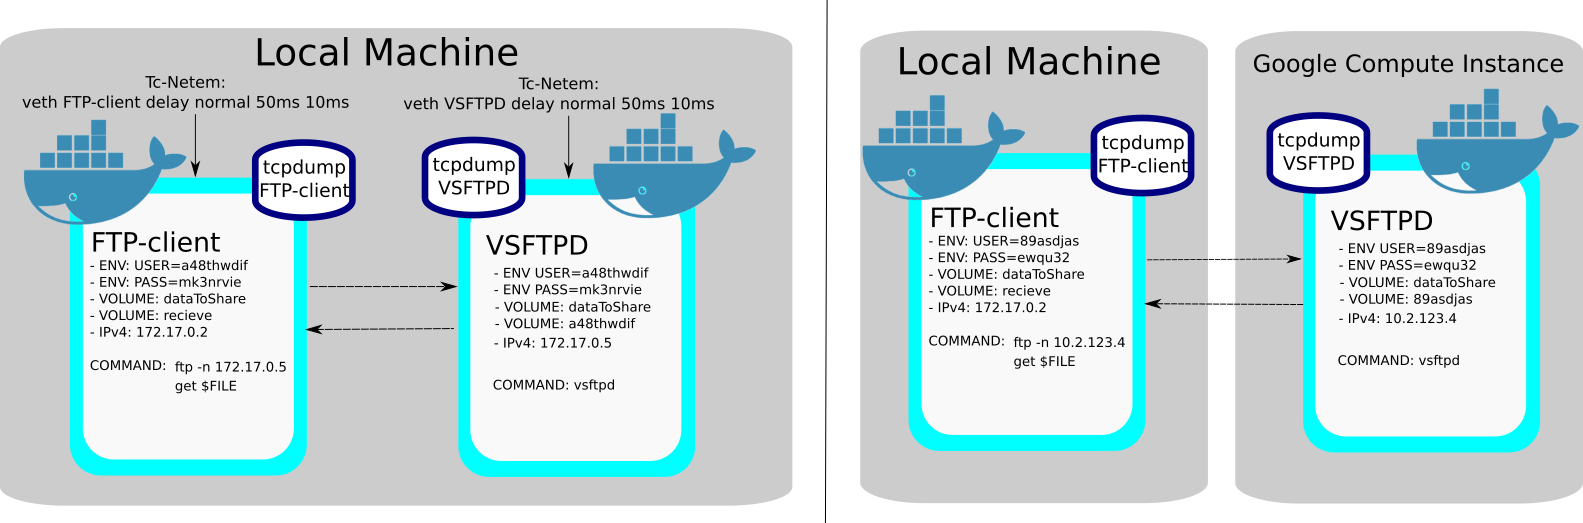
\includegraphics[width=14cm]{ftp_example_cloud.png}
\caption{\centering{Diagram showing how we generated our Local datasets (L) and our Google dataset (R)}}
\end{figure}

\texttt{tc-netem} allows for us to introduce packet delays according to a variety of distributions --- uniform, normal, Pareto and Paretonormal \footnote{This Paretonormal distribution is defined by the random variable $Z = 0.25*X + 0.75*Y$, where $X$ is a random variable drawn from a normal distribution and $Y$ is a random variable drawn from a Pareto distribution.}.  Initial testing revealed that a uniform distribution insufficiently modelled real-world traffic delays so we do not include it in our experimentation. Furthermore, \texttt{tc-netem} adds delays according to distribution tables and so it is relatively trivial to add our own. Therefore, after extracting the inter-arrival times of our Google dataset, we fit a Weibull distribution to this data before generating a \texttt{tc-netem} compatible distribution table. In total, we test the efficacy of four distributions to model inter-arrival times --- normal, Pareto, Paretonormal and Weibull.

We generate several Local datasets by delaying our traffic according these distributions, performing an exhaustive grid search over their means and standard deviations. For instance, one dataset consisted of our traffic delayed according to a normal distribution with a mean inter-arrival time of 50ms and a jitter of 20ms. Initial experimentation revealed that for all of our generated traffic, introducing delays with a mean in the range of 40ms to 70ms produced the best results. Thus, we limit our grid search to this range in 10ms intervals. Setting the jitter of the distribution too high resulted in the repeated arrival of packets out of order, therefore we further limit our grid search to jitter values in 5ms intervals up to half of the value of the mean. For instance, for a mean of 40ms, we consider jitter values of 5ms, 10ms, 15ms and 20ms. In total, we generate 88 Local datasets.

Our goal is to discover the Local dataset whose packet timings most closely resemble those of our Google dataset. To do this, we extract the IATs and packet sizes from our datasets on a packet-by-packet basis and store these results in arrays --- 250964 x 2 for our Google Dataset and roughly 245000 x 2 for all of our Local datasets. We measure the similarity between two of these arrays by training a Random Forest classifier to distinguish between them. We say that if the Random Forest correctly classifies each packet with a success rate of only 50\% then it is no better than randomly guessing and, as such, the inter-arrival times of these two arrays are indistinguishable from one another.

To perform this measurement, we concatenate one Local dataset array with our Google dataset array, label the entries and then shuffle the rows. We proportion this data into a training set and a testing set using an 80-20 split. We then feed this training data into a Random Forest with 1000 trees and fixed seed and then record the accuracy of this Random Forest on the test set. We repeat this process for every single Local dataset, 88 times in total.

\section{Experiment 2 - Classifying Application Flows using IATs}

\subsection{Motivation}

Having examined whether our Docker framework is capable of emulating real-world IATs, we explore their utility in traffic classification in depth. 

Classifying traffic based on IATs falls under the category of Stateful Packet Inspection (SPI), which attempts to segregate flows by examining only the first header and statistical characteristics of packets. Although SPI considers strictly less information about packets compared to DPI, this can be advantageous as it doesn't incur the high computation overheads of DPI, can classify encrypted traffic and produces fewer privacy concerns. Efficient traffic classification is essential for IDSes as this facilitates the detection of protocols running on atypical ports or unusual traffic patterns in real-time, which may indicate the presence of an intruder.

As network conditions vary considerably, machine-learning techniques for traffic classification are a fruitful approach with many successful published classifiers. Furthermore, inter-packet arrival times have been shown to be a discriminative feature \cite{zander2005automated} \cite{nguyen2008survey}. However, many of these methods classify completed flows and, therefore, consider statistical information about the IATs --- such as the mean and variance. However, on-the-fly classifiers are also successful. Jaber et al. \cite{jaber2011can} showed that a K-means classifier can classify flows in real-time solely based on IATs with precision exceeding 90\% for most protocols within 18 packets. Similarly, Bernaille et al. \cite{bernaille2006traffic} demonstrated that a K-means classifier can precisely classify traffic within five packets using only packet size as a feature. 

These results are promising for an IDS using IATs to classify malicious traffic. However, Jaber et al. only evaluated their traffic classifier with training and testing data drawn from the same dataset containing traces of a single network; there is no measure of how this model may generalise to other networks with differing conditions. Furthermore, they were limited to using unsupervised machine learning algorithms to classify their traffic as their datasets had no ground truth. 

We attempt to replicate these results within our Docker framework with some adjustments. As we can generate a fully accurate ground truth, we attempt to segregate application flows based on their IATs using supervised learning techniques. Moreover, we then measure this model's ability to generalise by testing its efficacy on another dataset with different network conditions.

\subsection{Data \& Preprocessing}

Our goal is to measure a classifier's ability to generalise across datasets. Therefore we construct two datasets using our Docker framework, both containing the same number of network traces from the same containers. 

For our first dataset, we generate 3200 .pcap files, each containing traffic from one of 16 different classes: HTTP (Client \& Server), HTTPS (Client \& Server), RTMP (Client, Server \& Viewer), SSH (Client \& Server), FTP (Client \& Server), IRC (Client \& Server), SMTP, SQLi and DoS traffic. To prevent class imbalance, we generate 200 examples for each class. To more accurately emulate potential network conditions, we use our \texttt{tc-netem} scripts to apply a unique delay to every container involved in a scenario. These delays follow a Pareto distribution with random mean between 0 and 100 milliseconds and random jitter between 0 and 10 milliseconds. We then preprocess this data by removing all but the first 12 packets of each .pcap file using \texttt{Editcap}. We extract the inter-arrival times of each packet and store the results for each class in a 11 x 200 array before concatenating a column of labels. We subsequently concatenate all of these 12 x 200 arrays together before shuffling the rows. We call this our \textit{Primary} dataset.

We then repeat this process to generate a second dataset, changing the properties of our emulated network. Again, we delay all traffic using a Pareto distribution, however, this time we select a random mean in the range of 100 to 500 milliseconds and random jitter between 0 and 50 milliseconds. The subsequent preprocessing of our data remains unchanged. We call this our \textit{Secondary} dataset.

\subsection{Methodology}
\label{sec:exp2_method}
First, we attempt to reproduce the results presented by Jaber et al. by training a Random Forest with 100 trees to classify application flows based off of packet IATs. We do this by proportioning our Primary dataset into training and testing sets using an 80-20 split. We then train and test our Random Forest repeatedly, first considering the classification accuracy based on the IATs of only the first two packets, then the first three packets and so on, up to 12 packets. We record the resulting confusion matrix for each round and calculate the precision and recall rates of our classifier.

Having trained our classifier, we measure its ability to generalise by repeating the above experiment, but replacing the test set with our Secondary dataset. Again, we record the precision and recall rates.

\section{Experiment 3 - Varying levels of Malicious Traffic}

\subsection{Motivation}

As discussed in section \ref{sec:datasets}, a consistent problem with existing network traffic datasets for intrusion detection is the difficulty in establishing the malicious traffic that the dataset should contain. Pendlebury et al. \cite{Pendlebury:2018:EFM:3243734.3278505} identify two ways in which the malicious traffic can be lacking: \textit{temporal} bias and \textit{spacial} bias. Temporal bias refers to the same phenomenon that Allix et al. \cite{allix2014machine} discuss; the classification accuracy of machine-learning anomaly detectors disimproves over the course of its deployment lifecycle as new malware and intrusion techniques begin to emerge. Spacial bias refers to unsound assumptions about the ratio of malicious traffic to benign traffic in the data. Many existing datasets in security over-represent the amount of malicious samples considerably.

Failing to account for these biases can vastly inflate the supposed performance of machine-learning based anomaly detectors \cite{pendlebury2019tesseract}. For instance, there exists numerous papers for numerous machine-learning algorithms boasting accuracy rates of 95\% or higher. However, these implementations often lack temporal robustness or, as discussed by Axelsson \cite{axelsson2000base}, fail to account for the \textit{base-rate fallacy}. This states that, because there exists a considerable class imbalance in network traffic --- that is, benign traffic vastly outnumbers malicious traffic ---, the effectiveness of intrusion detectors are limited by their false positive rate.

It is difficult to get a reasonable understanding of how spatial bias affects the efficacy of machine-learning-based intrusion detectors using existing datasets because of the high ratio of benign to malicious traffic. This means that if one wanted to investigate the effects spacial bias where, say, 50\%  of the training and testing data is malicious, it's necessary to either oversample malicious traffic or undersample benign traffic. However, these are both problematic; oversampling results in a considerable amount of duplicated data, which will patently inflate the accuracy of an intrusion detector. To prevent exact duplication, this data could be altered slightly but it's unclear whether this manipulated data actually resembles something that can be found in the real-world. Similarly, undersampling involves discarding a tremendous amount of benign data and, therefore, it is unclear whether one attains an accurate false positive rate --- it is possible that one has discarded entire classes of benign data.

However, generating data using our Docker framework does not suffer from these problems because, instead of oversampling, one can simply just generate more malicious traffic. To demonstrate this, we dedicate our second experiment to the exploration of spacial bias.

\subsection{Data \& Preprocessing}

In order to investigate the effects of spacial bias in intrusion detection datasets, we construct two datasets from our Docker framework --- one consisting of benign traffic and one consisting of malicious traffic. To create our benign dataset, we follow the design principals outlined in section \ref{sec:dataset_create}, resulting in a dataset consisting of roughly 80,000 flows of HTTP, DNS, SSL, FTP, SMTP, NTP and MySQL traffic. This contained 11.2 Gigabytes of traffic captured over the course of 22 hours. For our malicious dataset, we capture traffic originating from DoS, SQL injection, Url Fuzzing, SSH password bruteforcing and Heartbleed attacks. Again, this data consists of roughly 80,000 flows. In order to more closely resemble real-world traffic, any network traffic originating from the Docker virtual network was delayed according to a Pareto distribution with random mean and jitter. We then extracted the flow statistics from these two datasets using the CICFlowMeter tool \cite{netflowmeter}, which produces a CSV file of 80 different flow statistics that we use as features to train our machine-learning algorithms. These flow statistics are then normalised to lie between 0 and 1. We label all benign flows as 0 and all malicious flows as 1.

We use this data to create a further 12 training and test datasets --- six of each --- with various levels of spacial bias. In total, we had 6 distinct training and test sets containing 5\%, 10\%, 20\%, 40\%, 60\% and 80\% malicious traffic. Regardless of the amount of malicious traffic in the datasets, we ensured that the total number of flows in each dataset was fixed with our training datasets containing 60,000 flows and our test datasets containing 20,000 flows.

\subsection{Methodology}

To investigate the effects of spacial bias in intrusion detection datasets, we focus on two machine-learning algorithms that have reportedly produced excellent results in this domain: Random Forests and Multi-Layered Perceptrons (MLPs). We consider a random forest with 1000 trees and an MLP with three layers, each with 80 nodes. First, we fix the percentage of malicious traffic in the \textit{training} dataset to 5\% and 80\% before training our algorithms and calculating the resultant confusion matrix for all of our test datasets. We then repeat this process, fixing the percentage of malicious traffic in the \textit{test} datasets at 5\% and 80\% and training our algorithms using all of our training datasets and calculating the resultant confusion matrices.

%----- This experiment could probably be improved by including the results from upsampling malicious traffic from like UNSW or CIC-IDS. I have the scripts to do that easily and it pretty clearly demonstrates why upsampling doesn't work for this experiment, as you basically just get perfect results.


\chapter{Evaluation \& Results}
\label{sec:eval}

\section{Evaluation of Docker Scenarios \& Dataset}

The primary objective of this dissertation was the development of a series of scripted scenarios to generate both benign and malicious traffic from a variety of Docker containers. Moreover, we aimed to coalesce that traffic into a dataset for the purposes of training intrusion detection systems that had comparable qualities to existing datasets.

\subsection{Docker Scenarios}
\label{sec:docker_results}
Over the course of this project, we increase the number of Docker scenarios in the Detlearsom project by 17 for a total of 26 scenarios. Here, we evaluate our scenarios against the requirements discussed in section \ref{sec:require}.

\paragraph*{Coverage of Protocol Types}

We introduced several new protocols and applications flows to the Detlearsom project, including BIttorrent, DNS, X509, MySQL, NTP, RTMP and audio streaming. Of the datasets we listed in \ref{tab:results-bro}, we can use Detlearsom scenarios to generate datasets containing the protocols that make up at least 87.8\% of Mawi, 98.3\% of CIC-IDS 2017, 65.6\% of UNSW-NB15 and 94.5\% of ISCX Botnet benign IPv4 flows. Furthermore, we can generate traffic for which there is no equivalent in some of these datasets, such as RTMP or Bittorrent.

\paragraph*{Variation within Protocols}

In total, our scenarios have 40 variations. Examples of variations include launching 3 different DDoS attacks in our Mirai scenario, downloading websites using 4 different user-agents in our wget over WAN scenario and being able to launch both successful and unsuccessful attacks in our insecure SQL scenario. Of the scenarios that don't have explicitly coded variations, we ensure that we generate traffic with some variety to it, such as our RTMP scenario streaming one of several different video files.

\paragraph*{Inclusion of Malicious Traffic}

Our malicious scenarios cover a wide range of potential attacks. The majority of these are present in existing datasets, but we have also implemented many modern attacks that have no equivalent representation in other datasets, such as cryptojacking and XXE. Furthermore, our attacks span a considerable breadth of attack classes, including DoS, DDoS, CNC traffic, bruteforcing, web attacks and data exfiltration, as we aimed for. In total, we developed 11 malicious scenarios, covering 7 attack classes.

\paragraph*{Deterministic Scenarios} 
\vspace{-5mm}

\begin{figure}[H]
    \centering
    \begin{minipage}{0.5\textwidth}
        \centering
        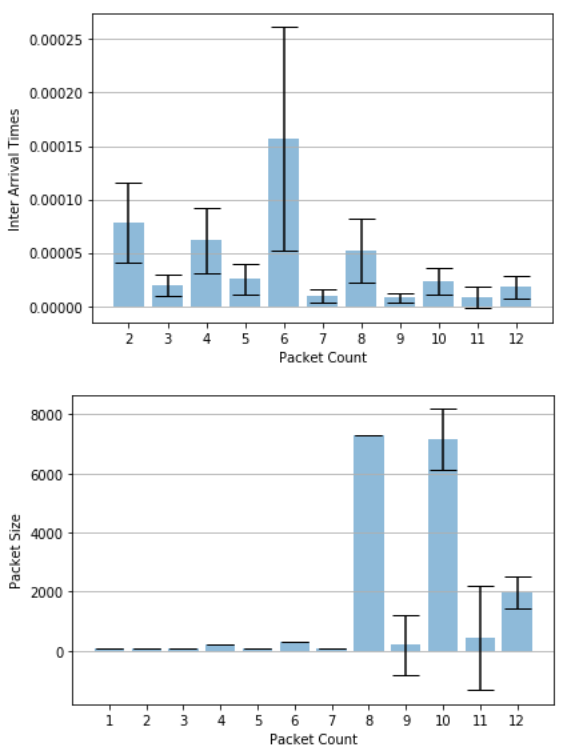
\includegraphics[width=0.8\textwidth]{test.png} % first figure itself
        \caption{\centering{Means of IATs \& Packet Sizes for Packets 1-12}}
        \label{fig:size1}
    \end{minipage}\hfill
    \begin{minipage}{0.5\textwidth}
        \centering
        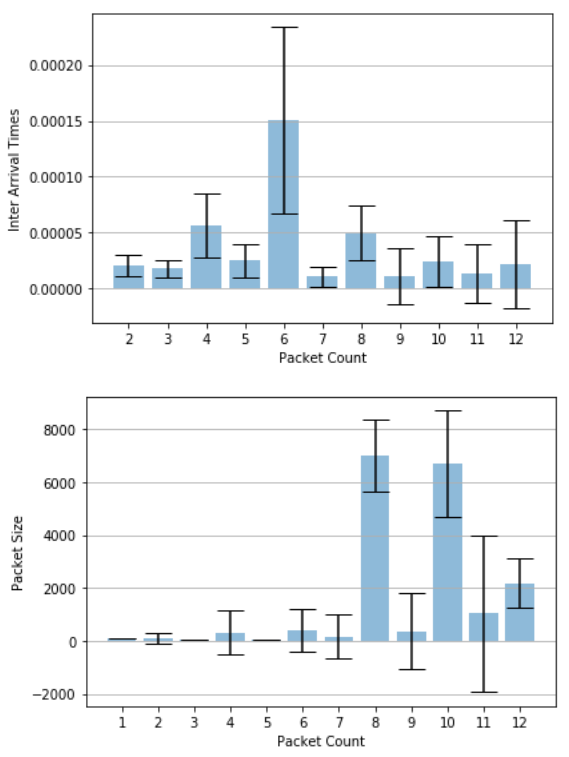
\includegraphics[width=0.8\textwidth]{time_variation_500.png} % second figure itself
        \caption{\centering{Means of IATs \& Packet Sizes for Packets 501-512}}
        \label{fig:size501}
    \end{minipage}
\end{figure}

To get some measure of how deterministic our scenarios are, we use our Apache scenario to generate 500 .pcap files containing  HTTP traffic. We apply no delays to the traffic and ensure that no other major processes are running during the capture so that there is minimal interference with the Docker virtual network. We then calculate the mean IATs and sizes of packet 1-12, seen in figure \ref{fig:size1} and packets 501-512, seen in figure \ref{fig:size501}. As we predicted in Section \ref{sec:deterministic}, a significant amount of our packets differ only minimally in timing, with size and content remaining fixed across datasets. Furthermore, we see periods of greater variation in packet sizes, as expected. This is caused by the non-deterministic nature of the Docker Virtual Ethernet and Apache, where the number of data packets following a TCP ACK can vary. As such, we verify that our scenrios are deterministic up to networking and computational differences.


\paragraph*{Automated Capture}

Upon running their respective startup scripts, all of our scenarios launch the needed containers, proceed with the specified scenario, capture all traffic and then take down all containers and networks. Moreover, our scenarios are ephemeral; we can run each scenario repeatedly with no additional configuration.

\subsection{Dataset}
\vspace{-5mm}
\captionof{table}{\label{tab:dataset}}
\begin{tabular}{ |p{2cm}||p{2cm}| {p3cm} | p{2.75cm} | p{2cm} |  p{1.8cm} | }
 %\hline
 %\multicolumn{5}{|c|}{} \\
 \hline
 Name & \# Variations & \# Files \& Size  & Complete Capture? &  Total Interaction? & Labelled?\\
 \hline
Wget WAN & 6 & 160 \& 20.1GB & $\sqrt{}$ &  &  $\sqrt{}$ \\
Bittorrent & 1 & 12 \& 1.2GB & $\sqrt{}$ &  &  $\sqrt{}$ \\
SQL & 1 & 50 \& 536.2MB & $\sqrt{}$ & $\sqrt{}$ &  $\sqrt{}$ \\
Apache & 2 & 36 \& 30MB & $\sqrt{}$ & $\sqrt{}$ &  $\sqrt{}$ \\
Nginx & 2 & 36 \& 33.8MB & $\sqrt{}$ & $\sqrt{}$ &  $\sqrt{}$ \\
FTP & 12 & 68 \& 305.6MB & $\sqrt{}$ & $\sqrt{}$ &  $\sqrt{}$ \\
SSH & 2 & 40 \& 109MB & $\sqrt{}$ & $\sqrt{}$ &  $\sqrt{}$ \\
RTMP & 1 & 33 \& 573.5MB & $\sqrt{}$ & $\sqrt{}$ &  $\sqrt{}$ \\
NTP & 1 & 60 \& 142KB & $\sqrt{}$ &  &  $\sqrt{}$ \\
SMTP & 2 & 50 \& 49MB & $\sqrt{}$ &  &  $\sqrt{}$ \\
Goldeneye & 1 & 2 \& 523MB & $\sqrt{}$ & $\sqrt{}$ &  $\sqrt{}$ \\
SSH BF & 2 & 4 \& 120MB & $\sqrt{}$ & $\sqrt{}$ &  $\sqrt{}$ \\
URL Fuzz & 1 & 6 \& 35.2MB & $\sqrt{}$ & $\sqrt{}$ &  $\sqrt{}$ \\
SQLi & 1 & 15 \& 70MB & $\sqrt{}$ & $\sqrt{}$ &  $\sqrt{}$ \\
XXE & 2 & 4 \& 12MB & $\sqrt{}$ & $\sqrt{}$ &  $\sqrt{}$ \\
Mirai & 1 & 6 \& 1.6GB & $\sqrt{}$ & $\sqrt{}$ &  $\sqrt{}$ \\
Heartbleed & 1 & 20 \& 40MB & $\sqrt{}$ & $\sqrt{}$ &  $\sqrt{}$ \\
 \hline
\end{tabular}


We combine 574 .pcap files using the methodology outlined in section \ref{sec:dataset_create} to create a network intrusion dataset totalling 24.8 Gigabytes.  We extract the flow features from this data using the CICFlowMeter tool \cite{netflowmeter}, creating flow statistics for over 300000 flows. Here, we evaluate this dataset according to the standards we outlined in section \ref{dataset_require}. We provide an overview of this dataset in table \ref{tab:dataset}. Note that providing Total Interaction is not applicable to some of our scenarios as they do not produce LAN traffic.

All of the traffic in our dataset has had artificial delays introduced according to a Pareto distribution with random mean between 0m and 200ms and random jitter between 0ms and 50ms. As shown in section \ref{sec:exp1_res}, this particular configuration accurately resembles realistic network conditions and produces data that is largely indistinguishable from real-world traffic. Thus, we satisfy the \textit{Realistic Network and Traffic} requirement. Furthermore, we include 6 different attack types, satisfying the \textit{Diverse Intrusion Scenarios} requirement. 



\subsubsection{Difficulties \& Limitations}

A great deal of the challenge of developing these scenarios came from the restrictions of the Docker framework. In particular, this meant that in order to get each container in a functioning state, a tremendous amount of configuration was necessary. Although many services that are commonly used in conjunction with Docker are maintained by official developers, many of the more obscure applications used in this project do not, leading to a spate of errors. Furthermore, these problems were often unique to that particular service being used in Docker and therefore documentation was non-existent. These problems were compounded further by the atypical manner in which we were using containers to communicate with one another.

As an example, many issues arouse when developing the bittorrent scenario using the linuxserver/transmission image. Although this image is both popular and maintained by a dedicated community, our usage differed significantly enough to cause several bugs. Usually, the linuxserver/transmission image acts as a server to provide a web GUI for viewing the status of torrents residing on the host machine. In contrast, we wanted the process of creating, downloading and seeding torrents to be contained entirely within the Docker container with no usage of the web GUI. However, this results in an immediate problem when creating torrent files. Each torrent file should contain information pertaining to the location of the information that's to be shared; however, when the torrent file is created in a Docker container and then pushed to the transmission server, transmission fails to recognise that the location specified in the file is accessible from the Docker container. As such, transmission attempts to download the file instead of seeding it, despite having full ownership over it already. Unfortunately, this problem seems to be universal across any implementation for creating torrent files from the command line usuable in Docker. In attempting to fix this issue, we tried using \texttt{mktorrent}, \texttt{buildtorrent}, \texttt{ctorrent} and \texttt{py3createtorrent}, each of which necessitated rebuilding most of the images of the scenario, but none worked. Finally, in order to get it working, we decided to relax our design criteria for this particular scenario, requiring that transmission must also be installed on the host machine. This allows for torrents to be created on the host machine before transmitting them to the Docker container, which resolves the issue.




\section{Results of Experiment 1}
\label{sec:exp1_res}
\vspace{-5mm}
\begin{figure}[hb!]
\captionsetup{justification=centering}
\centering
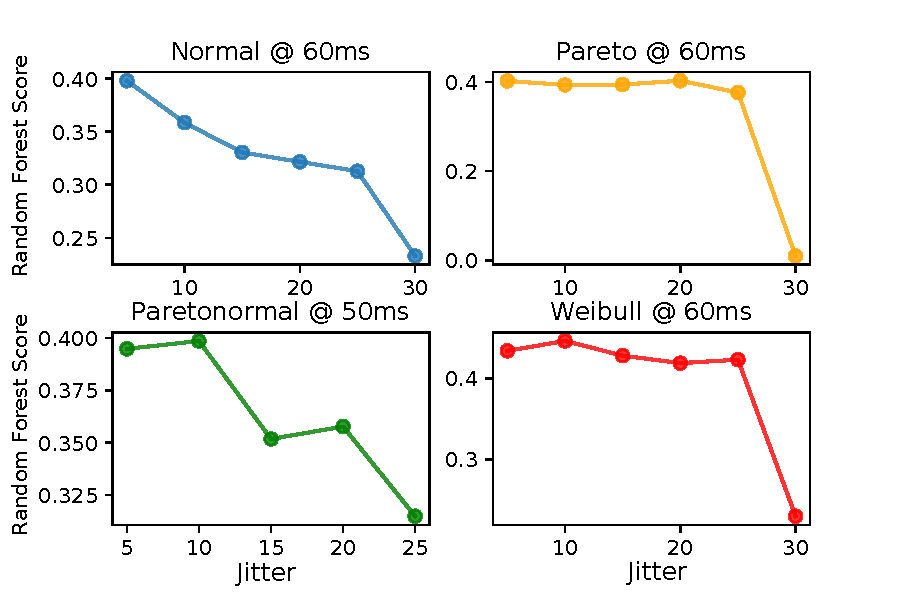
\includegraphics[width=120mm]{rf_results_with_label.pdf}
\caption{Results of Random Forest Classifier for a given distribution at the best performing delay - Note that a score of .5 represents 'perfect' indistinguishability}
\label{fig:rf_graph}
\end{figure}

\begin{table}[ht!]
\begin{center}
\begin{small}
\begin{sc}
\begin{tabular}{ccccc}
\hline
\abovespace\belowspace
Distribution & Mean & Jitter & RF Accuracy\\
\hline
\abovespace
No Delays (Baseline)         & 0          & 0ms         & 0.8176                 \\
Constant Delay          & 40ms          & 0ms         & 0.6730                 \\
Normal          & 60ms          & 5ms          & 0.6028                \\
Pareto          & 60ms          & 10ms          & 0.5979                \\
Paretonormal          & 50ms          &  10ms         & 0.6015                \\
\belowspace
Weibull          & 60ms          & 10ms          & 0.5540               \\
\hline
\end{tabular}
\end{sc}
\end{small}
\vskip -2mm
\caption{Worst Random Forest accuracy rates for a given distribution}
\label{tab:results-iat_rf}
\end{center}
\vskip -4mm
\end{table}

Table \ref{tab:results-iat_rf} summarises the values of the mean and jitter for a given distribution that produced the worst results from the random forest classifier.

In order to establish a baseline, we first compare the traffic generated from our Docker scenario to that of the Google Compute data with no added delays. In this case, our Random Forest was largely able to distinguish between the two datasets, achieving an accuracy of over 80\%. As can be seen, the classification accuracy is worsened considerably by introducing a constant delay to the packets, ensuring that the mean IAT of the two datasets are roughly similar. This was then further worsened by introducing network delays according to all of our tested distributions.

Although the best performing results of the Normal, Pareto and Paretonormal distributions are largely similar, we note that, as can be seen in figure \ref{fig:rf_graph} that increasing the jitter steadily improved the performance of the random forest classifier. In contrast, the Pareto and Weibull distributions maintain low-levels of accuracy as jitter increases --- barring the highest values of jitter, due to the effect discussed in Section \ref{sec:method1}. This seems to be due to the fact that both the normal and Paretonormal distributions fail to fall off quickly enough to model the IATs of our Google dataset.



\begin{comment}

\begin{figure}[h!]
\centering
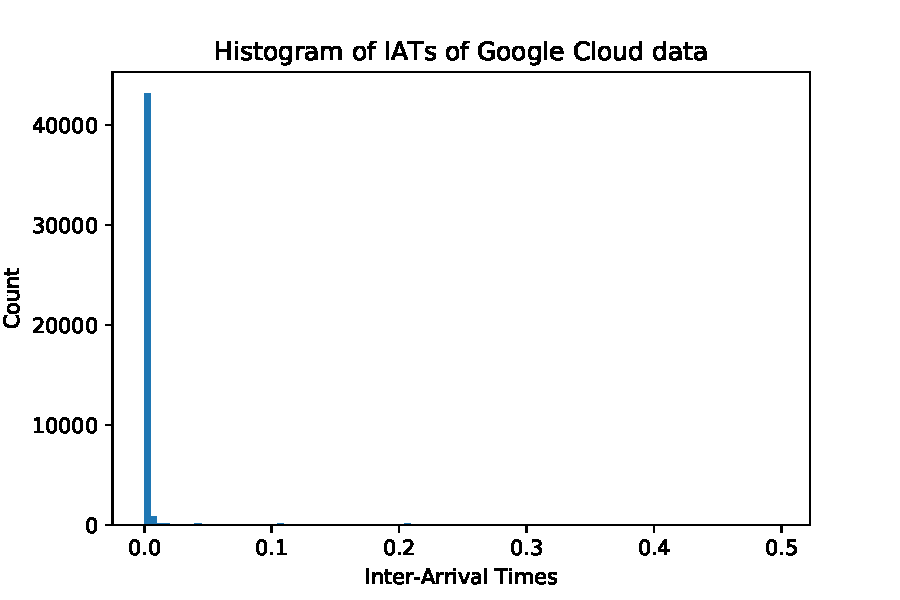
\includegraphics{IAT_g_server.pdf}
\end{figure}

\begin{figure}[h!]
\centering
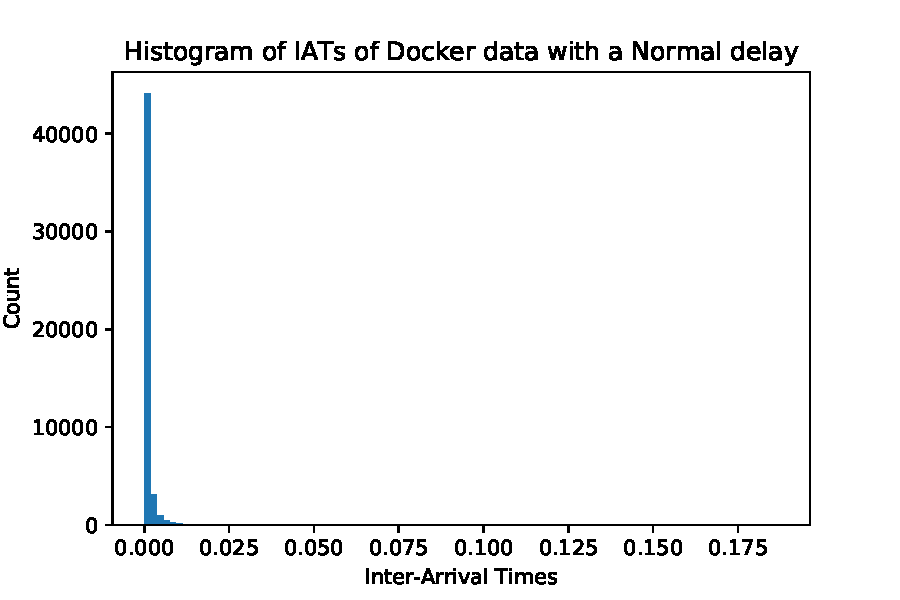
\includegraphics{iat_normal_delay.pdf}
\end{figure}

\begin{figure}[h!]
\centering
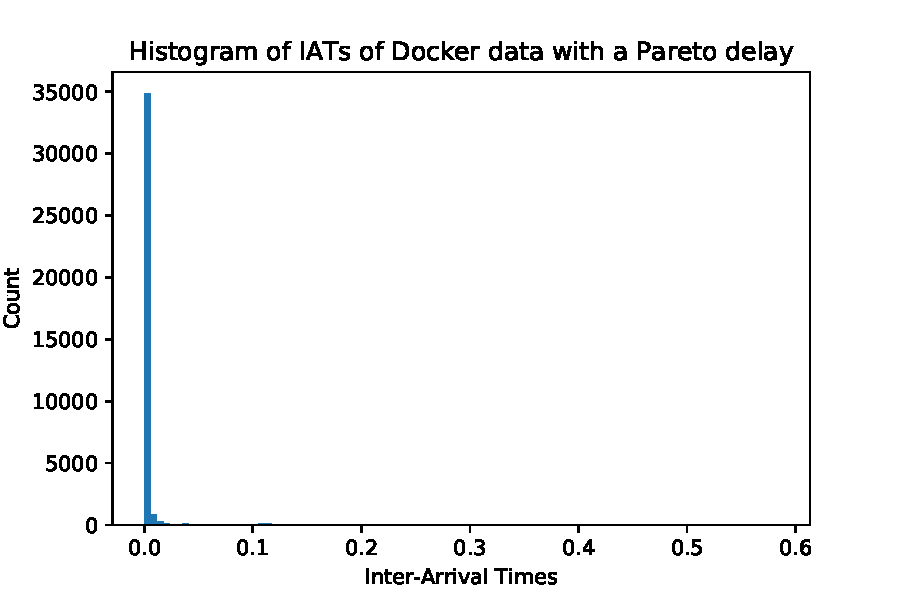
\includegraphics{iat_pareto_delay.pdf}
\end{figure}

\begin{figure}[h!]
\centering
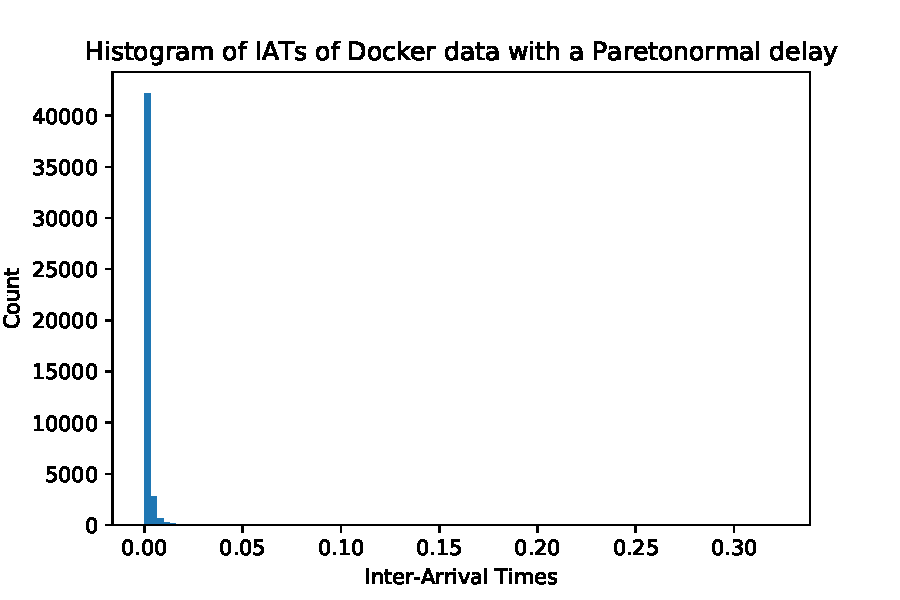
\includegraphics{iat_paretonormal_delay.pdf}
\end{figure}

\begin{figure}[h!]
\centering
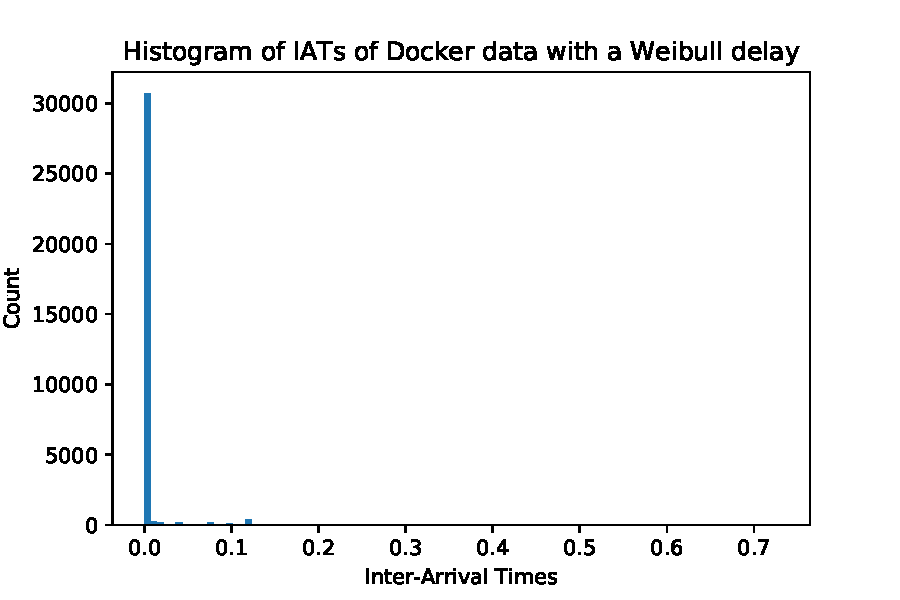
\includegraphics{iat_weibull_delay.pdf}
\end{figure}

\end{comment}

\section{Results of Experiment 2}

\vspace{-7mm}
\begin{figure}[H]
    \centering
    \begin{minipage}{0.5\textwidth}
        \centering
        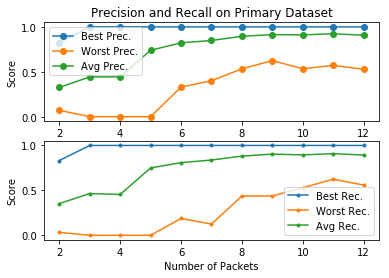
\includegraphics[width=0.9\textwidth]{primary_prec.png} % first figure itself
        \caption{\centering{Precision \& Recall for Primary Dataset}}
        \label{fig:primary}
    \end{minipage}\hfill
    \begin{minipage}{0.5\textwidth}
        \centering
        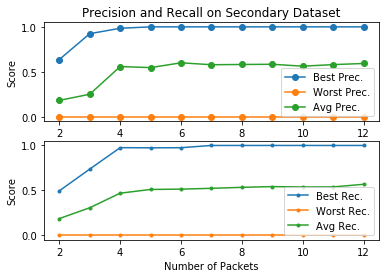
\includegraphics[width=0.9\textwidth]{secondary_prec.png} % second figure itself
        \caption{\centering{Precision \& Recall for Secondary Dataset}}
        \label{fig:secondary}
    \end{minipage}
\end{figure}

 After each run of our Random Forest on our Primary dataset, we gather the True Positive ($T_{P}$), False Positive ($F_{P}$) and False Negative ($F_{N})$ rate for each class. We then calculate their precision --- defined as $ \frac{T_P}{T_P + F_P}$ --- and recall --- defined as $ \frac{T_P}{T_P + F_N}$ --- values. in figure \ref{fig:primary}, we see that our average precision and recall across the classes exceed 0.9 after 10 IATs. However, our classifier had some difficulty distinguishing between certain, interrelated classes: in particular, we achieve a maximum precision and accuracy of only 0.5714 and 0.625 respectively on our RTMP-streamer class. This is because many of these features were incorrectly labelled as being from the RTMP-server class. This is the only server-client pair that suffered from this inaccuracy. Furthermore, after 12 packets our DoS and SQLi data is classified with precision and recall rates of 1.0 and 1.0 and 0.9462 and 0.9322 respectively.

This does not hold when we test our Random Forest on our Secondary dataset. As seen in figure \ref{fig:secondary}, we see a substantial decrease in our average precision and recall rates, achieving a maximum of 0.5923 and 0.5676 respectively. Moreover, after four packets, increasing the number of IATs in our dataset provides little additional benefit. Although some services generalised well, such as IRC-client and IRC-server, others failed to be classified, with every single SMTP feature being classified as HTTP-client. We also see a substantial drop-off in the classification of malicious traffic, with the precision rates of DoS and SQLi data not exceeding 0.6.

\section{Results of Experiment 3}
\vspace{-5mm}
\begin{figure}[H]
\begin{tabular}{h!}
  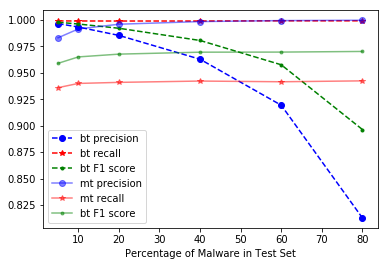
\includegraphics[width=60mm]{rf_5_train_legend.png} &   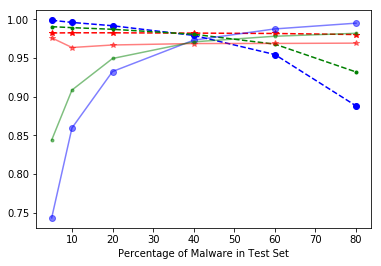
\includegraphics[width=60mm]{mlp_5_train.png} \\
(a) RF: Trained @ 5\% malicious traffic & (b) MLP: Trained @ 5\% malicious traffic \\[6pt]
 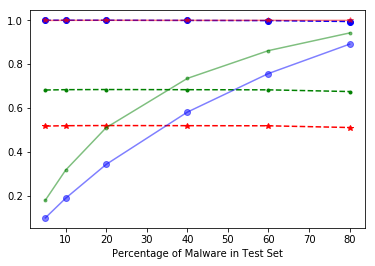
\includegraphics[width=60mm]{random_forest_80_train.png} &   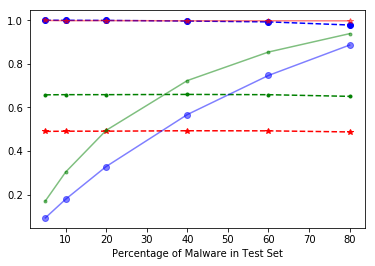
\includegraphics[width=60mm]{MLP_80_train.png} \\
(c) RF: Trained @ 80\% malicious traffic & (d) MLP: Trained @ 80\% malicious traffic \\[6pt]
\end{tabular}
\caption{Spacial Bias in Training Set}
\label{fig:test_bias}
\end{figure}

\begin{figure}
\begin{tabular}{h!}
  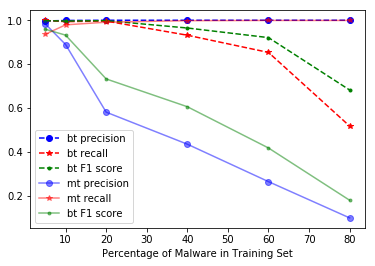
\includegraphics[width=60mm]{rf_5_test_legend.png} &   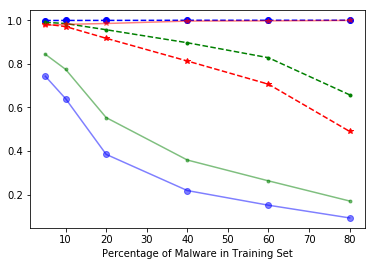
\includegraphics[width=60mm]{mlp_5_test.png} \\
(a) RF: Tested @ 5\% malicious traffic & (b) MLP: Tested @ 5\% malicious traffic \\[6pt]
 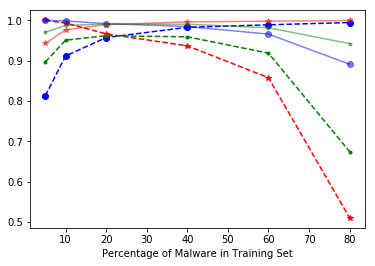
\includegraphics[width=60mm]{rf_80_test.png} &   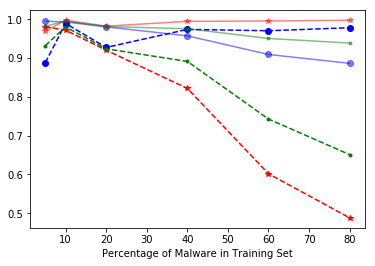
\includegraphics[width=60mm]{mlp_80_test.png} \\
(c) RF: Tested @ 80\% malicious traffic & (d) MLP: Tested @ 80\% malicious traffic \\[6pt]
\end{tabular}
\caption{Spacial Bias in Test Set}
\label{fig:train_bias}
\end{figure}

\vspace{-3mm}

Having trained our algorithms several times, we gather the number of True Positives ($T_P$), True Negatives ($T_N$), False Positives ($F_P$) and False Negatives ($F_N$). We then calculate the recall, precision and $F_1$-score for both the benign and malicious traffic.  We produce two sets of graphs from our results, figure \ref{fig:test_bias} and figure \ref{fig:train_bias}, demonstrating the effects of spacial bias in the testing and training datasets respectively.

To begin, consider the results for malicious traffic in figure \ref{fig:test_bias}. We note that the anomaly precision ($P_{mt}$) steadily increases as the percentage of malicious traffic in the test set increases. In contrast, anomaly recall ($R_{mt}$)  remains steady. This is due to the decreasing amount of benign traffic in the dataset and, therefore, the effect is most sharply pronounced when there is a large amount of malicious traffic in the training set. Note that the $F_1$-score is a function of $P_{mt}$ and $R_{mt}$ --- $F_1 = 2*\frac{P_{mt} * R_{mt}}{P_{mt} + R_{mt}}$ --- and therefore increases with precision. In contrast, there is a inverse relationship with the precision of the benign traffic classification --- where $P_{bt} = \frac{T_N}{T_N + F_N}$. This is because our false negatives increase whilst our true negatives decrease as we increase the amount of malicious traffic in the test set. Similarly, consider the effects of spacial bias on the training dataset in figure \ref{fig:train_bias}. Although slight, we see increasing the amount of malicious traffic during training causes $R_{mt}$ to increase as $P_{mt}$ degrades. This is caused by the number of false negatives increasing whilst the number of true positives remains sturdy. Again, as  with testing bias, there is an inverse relationship with the recall rates of benign traffic, whilst precision increases or remains steady.




\chapter{Conclusions}
\label{sec:conc}

\section{Discussion of Experiments}

\paragraph*{Experiment 1} We designed this experiment with the aim of demonstrating that our Docker framework can produce traffic that is sufficiently similar to that found in the real-world. From the results, we conclude two things. Firstly, we confirm that, for this particular experiment, the research discussed in section \ref{sec:IATs} holds and that both the Pareto distribution and the Weibull distribution most accurately model real-world IATs. Secondly, we demonstrate that by introducing artificial network delays to our docker virtual network, it is possible to reasonably approximate the IATs of real-world traffic, with our Random Forest mistakenly classifying 40\% of our Docker traffic when delayed according to a Pareto distribution and 45\% when delayed according to a Weibull distribution. We stress the importance of this result; if our Random Forest could more easily distinguish between our classes, then the utility of our framework is questionable as we could not produce realistic traffic.

\paragraph*{Experiment 2} When our Random Forest classifier is tested on traffic produced with the same network conditions as the training set, we reproduce the results of Jaber et al.\cite{jaber2011can}. We similarly find that our average precision and recall values quickly rise to above .75 within 5 IATs before levelling off and achieving values exceeding 0.9 by 11 IATs. However, we see that this Random Forest does not generalise well when tested on traffic with different network conditions. We see a substantial loss in the average precision and recall rate, achieving maximal values of 0.5923 and 0.5676 respectively.

This experiment highlights a major difficulty in training traffic classification systems; it is vitally important that network intrusion datasets contain traffic from a wide variety of network conditions. This is concerning for intrusion detection, as our Random Forest failed to classify DoS and SQLi data with meaningful accuracy.


\paragraph*{Experiment 3}

We reproduce the results found by Pendlebury et al. \cite{pendlebury2019tesseract}, verifying that spacial bias in either the training or testing sets causes an inverse relationship between the precision and recall rates of benign traffic and malicious traffic. We feel this experiment particularly exemplifies the advantages of our Docker framework; since we can repeatedly generate  datasets with arbitrary ratios of benign to malicious traffic, we don't have to upsample or downsample either class to simulate spacial bias, both of which can lead to inaccurate assessments of a classifier's precision and recall rates. 

\section{Conclusion, Criticism \& Future Work}


In order to protect both networks and users from harm, the development of IDSes is of vital importance. However, presently, the lack of quality, expandable datasets with accurate ground truths limits the value of machine-learning-based anomaly detection. The primary goal of this project was the creation of a Docker framework capable of generating worthwhile network intrusion datasets that satisfy these conditions. To do so, we designed and implemented 17 containerised scenarios capable of producing benign and malicious network traces, coalescing this traffic into a dataset. We also demonstrated that it is possible to introduce artificial delays to the Docker virtual network such that it meaningfully resembles a wide-area network. Following this, to exhibit the advantages of our data generation framework, we performed two experiments that would be difficult to accomplish using standard, static datasets.

We generated a large network intrusion dataset but we don't perform any testing or experimentation with it. Ultimately, it proved too difficult to implement our framework, generate large amounts of data and design a novel intrusion detection system all within the time frame of the dissertation. Instead, this dataset serves as an example of what is possible using our Docker scenarios.

As our Docker framework is designed to be expandable, there are many avenues for future work. One  possibility would be to simply continue developing Docker scenarios to include greater protocol variety and attack diversity. Alternatively, the scenarios could be expanded to include IPv6 traffic. The functionality of the scenarios could also be expanded to capture log data as well as network traffic, providing an additional source of features for IDS training \cite{abad2003log}.



\bibliographystyle{plain}
\bibliography{mybibfile}

%% You can include appendices like this:
 \appendix
% 
 \chapter{Secure SQL Code}
% 
\section{Docker-Compose.yml}
  \begin{minted}[
    gobble=4,
    frame=single,
    linenos
  ]{yaml}
    version: '2'

    services:
        sql:
            image: 'mysql/mysql-server'
            container_name: mysql
            ports:
              - '3306'
            volumes: 
              - $PWD/sql-share:/home/share/
              - $PWD/sql_settings/my.cnf:/etc/my.cnf
            networks:
                capture:
                    ipv4_address: 172.16.238.22
  
        apache:
            image: 'detlearsom/php'
            volumes:
              - '$PWD/config:/var/www/html'
            ports:
              - "80:80"
            networks:
                capture:
                    ipv4_address: 172.16.238.20

        admin_user:
            image: 'python-requests'
            command: python /usr/share/scripts/populate_userlist.py
            volumes:
              - '$PWD/admin-share:/usr/share/scripts'
            networks:
              - capture

        tcpdump_apache:
            image: 'detlearsom/tcpdump'
                command: not(ip6 or arp or (udp and
                (src port 5353 or src port 57621))) -v -w
                "/data/dump-150-apache-${CAPTURETIME}-$REPNUM.pcap"
            volumes:
              - '$PWD/data:/data'
            network_mode: "service:apache"
            depends_on:
             - dummy

        tcpdump_admin:
            image: 'detlearsom/tcpdump'
            command: not(ip6 or arp or (udp and
            (src port 5353 or src port 57621))) -v -w
            "/data/dump-150-admin-${CAPTURETIME}-$REPNUM.pcap"
            volumes:
                - '$PWD/data:/data'
            network_mode: "service:admin_user"
            depends_on:
              - dummy

        tcpdump_sql:
            image: 'detlearsom/tcpdump'
            command: not(ip6 or arp or (udp and
            (src port 5353 or src port 57621))) -v -w
            "/data/dump-150-sql-${CAPTURETIME}-$REPNUM.pcap"
            volumes:
              - '$PWD/data:/data'
            network_mode: "service:sql"
            depends_on:
              - dummy

        dummy:
            image: 'alpine'
            networks:
              - capture
            depends_on:
              - sql
              - apache
              - admin_user


    networks:
      capture:
        driver: "bridge"
        ipam:
          driver: default
          config:
              - subnet: 172.16.238.0/24
                gateway: 172.16.238.1
  \end{minted}

\section{Start-Up Script}


\begin{lstlisting}[language=bash]
#!/bin/bash

export DURATION="$1"
export CAPTURETIME=`date +%Y-%m-%d_%H-%M-%S`
REPEAT="$2"


[ -z "$DURATION" ] && DURATION=60
[ -z "$REPEAT" ] && REPEAT=1

function add_delays {
    echo "Adding delays to the network..."
    DELAY1=$((RANDOM % 100 + 1))
    DELAY2=$((RANDOM % 100 + 1))
    DELAY3=$((RANDOM % 100 + 1))

     # Our tc-netem scripts that add delays to network.
    ./container_tc.sh mysql $DELAY1
    ./container_tc.sh capture-140-securesql_apache_1 $DELAY2
    ./container_tc.sh capture-140-securesql_admin_user_1 $DELAY3
}



trap '{ echo "Interrupted."; teardown; exit 1; }' INT

for ((i=1; i<=REPEAT; i++))
do
    echo "Repeat Nr " $i
    export REPNUM=$i
    docker-compose up -d
    add_delays;
    sleep 60
    
    PREFIX="[Entrypoint] GENERATED ROOT PASSWORD: "
    FULL_PASS=$(docker logs mysql 2>&1 | grep GENERATED)
    FULL_PASS=${FULL_PASS#"$PREFIX"}
    echo "$FULL_PASS"
    docker exec -it mysql /home/share/sql_script.sh $FULL_PASS
    echo "Capturing data now for $DURATION seconds...."
    sleep $DURATION

    docker-compose down
done

\end{lstlisting}

\section{Login Page with Prepared Statements - Code Snippet}


\begin{lstlisting}[language=php, breaklines=true]

// Code taken/modified from https://www.tutorialrepublic.com/php-tutorial/php-mysql-login-system.php

$sql = "SELECT id, username, password FROM users WHERE username = ?";
// Prepare Statement
if($stmt = mysqli_prepare($link, $sql)){
    // Bind Variables to Statement
    mysqli_stmt_bind_param($stmt, "s", $param_username);

    $param_username = $username;

    // Execute the prepared statement
    if(mysqli_stmt_execute($stmt)){
        mysqli_stmt_store_result($stmt);

        // Check if username exists
        if(mysqli_stmt_num_rows($stmt) == 1){
            // Bind result variables
            mysqli_stmt_bind_result($stmt, $id, $username, $hashed_password);
            if(mysqli_stmt_fetch($stmt)){
                \\ Verify password
                if(password_verify($password, $hashed_password)){
                    // Start new session
                    session_start();

                    // Session variables
                    $_SESSION["loggedin"] = true;
                    $_SESSION["id"] = $id;
                    $_SESSION["username"] = $username;

\end{lstlisting}


\section{SQL Start-Up Script}


\begin{lstlisting}[language=bash, breaklines=true]

#!/bin/bash

PASS=$1

mysql  --connect-expired-password -uroot -p"$PASS" <<END_SCRIPT
ALTER USER 'root'@'localhost' IDENTIFIED WITH mysql_native_password BY 'password';
\q
END_SCRIPT

mysql --connect-expired-password -uroot -ppassword <<END_SCRIPT
CREATE DATABASE dbname;
CREATE USER 'admin'@'%' IDENTIFIED BY 'password';
ALTER USER 'admin'@'%' IDENTIFIED BY 'password';
GRANT ALL PRIVILEGES ON dbname.* TO 'admin'@'%';

FLUSH PRIVILEGES;

USE dbname;

CREATE TABLE users (
    id INT NOT NULL PRIMARY KEY AUTO_INCREMENT,
    username VARCHAR(50) NOT NULL UNIQUE,
    password VARCHAR(255) NOT NULL,
    created_at DATETIME DEFAULT CURRENT_TIMESTAMP
);


END_SCRIPT

\end{lstlisting}

% \section{First section}
% 
% Markers do not have to consider appendices. Make sure that your contributions
% are made clear in the main body of the dissertation (within the page limit).

\end{document}
